\documentclass[oneside,a4paper,openany,11pt]{ctexbook}

\usepackage{geometry}
\geometry{a4paper,left=2.0cm,right=2.0cm,top=2.5cm,bottom=2.2cm}

\usepackage{siunitx} % 物理单位
% \usepackage{tikz} % 画图宏包

\usepackage{graphicx}
\usepackage{amsmath,amsfonts,amssymb,amsthm}
\usepackage{slashed}
\usepackage{url}

\newcommand*{\dif}{\mathop{}\!\mathrm{d}} % 定义微分算子

%%%%% url 自动断词换行 %%%%%
\makeatletter
\def\UrlAlphabet{%
      \do\a\do\b\do\c\do\d\do\e\do\f\do\g\do\h\do\i\do\j%
      \do\k\do\l\do\m\do\n\do\o\do\p\do\q\do\r\do\s\do\t%
      \do\u\do\v\do\w\do\x\do\y\do\z\do\A\do\B\do\C\do\D%
      \do\E\do\F\do\G\do\H\do\I\do\J\do\K\do\L\do\M\do\N%
      \do\O\do\P\do\Q\do\R\do\S\do\T\do\U\do\V\do\W\do\X%
      \do\Y\do\Z}
\def\UrlDigits{\do\1\do\2\do\3\do\4\do\5\do\6\do\7\do\8\do\9\do\0}
\g@addto@macro{\UrlBreaks}{\UrlOrds}
\g@addto@macro{\UrlBreaks}{\UrlAlphabet}
\g@addto@macro{\UrlBreaks}{\UrlDigits}
\makeatother
%%%%% url 自动断词换行 %%%%%

\usepackage[breaklinks,colorlinks,linkcolor=black,citecolor=black,urlcolor=black]{hyperref}

\title{粒子物理学习笔记}
\author{HarryZ}
\date{\today}

\begin{document}

\maketitle

\chapter{粒子物理与量子场论}

\section{概述}

粒子物理学的理论基础是量子场论。

\subsection{自然单位制}

在粒子物理学中,为简便起见,经常采用自然单位制,取 $c=\hbar=k_B=1$

在自然单位制中,\emph{长度} 量纲与 \emph{时间} 相同,是 \emph{能量} 量纲的倒数,能量、质量、动量和温度具有相同量纲,可将能量单位电子伏特 $(\unit{eV})$ 视作唯一基本单位。

\subsection{有理化的自然单位制}

精细结构常数没有量纲,在任何单位制下的数值为 $1/137.036$

自然单位制 \emph{不可能} 将 $\hbar, c, \varepsilon_0$ 和 $e$ 这四个常数同时取为 $1$

粒子物理学中,时常取真空介电常数 $\varepsilon_0=1$,则真空磁导率 $\mu_0=\frac{1}{\varepsilon_0 c^2}=1$

\subsection{基本相互作用}

按照目前的认识,组成物质的基本单元是粒子,自然界中存在四种基本相互作用,支配着粒子的运动和转化。

\begin{enumerate}
    \item 引力相互作用
    \item 电磁相互作用
    \item 强相互作用
    \item 弱相互作用
\end{enumerate}

前两种是 \emph{长程} 相互作用,与日常生活联系最为密切。

\begin{itemize}
    \item 源:决定相互作用的种类
    \item 相互作用常数:决定相互作用的强度
    \item 媒介粒子:传递相互作用的粒子
    \item 力程:相互作用的有效范围
\end{itemize}

\subsection{引力相互作用}

\begin{itemize}
    \item 所有物质都参与引力相互作用
    \item 引力的源是质量,假想中的媒介粒子叫 \emph{引力子}
    \item 相互作用常数是牛顿引力常数:$\frac{G_N}{4\pi}=\qty{5.34e-40}{GeV^{-2}}$
    \item 引起的束缚态:行星系 (如太阳系)、恒星系 (如银河系)、星系团
    \item 目前尚未确立成熟的、得到实验检验的 \emph{量子引力理论}
\end{itemize}

\subsection{电磁相互作用}

\begin{itemize}
    \item 所有带电粒子都参与电磁相互作用
    \item 电磁相互作用的源是电荷,媒介粒子是光子
    \item 电磁相互作用常数是 \emph{精细结构常数}
        \begin{equation}
            \alpha = \frac{e^2}{4\pi} = \frac{1}{137.036}
        \end{equation}
    \item 引起的束缚态:原子、分子
    \item 19 世纪中叶,麦克斯韦将电和磁统一在电动力学的方程组中
    \item 20 世纪中叶建立起量子电动力学,它是第一个自洽的量子场理论
\end{itemize}

\subsection{强相互作用}

\begin{itemize}
    \item 原子核内部质子和中子 (统称核子) 之间的作用力可以抵消质子之间的同性电磁排斥力,使原子核稳定存在
    \item 核子间存在不同于引力和电磁相互作用的另一种相互作用,它的强度还强于电磁相互作用,称为强相互作用
    \item 描述强相互作用的基本理论是量子色动力学强相互作用的源是色荷,媒介粒子是胶子
    \item 相互作用常数是 \emph{强耦合常数}:$\alpha_s=\frac{g_s^2}{4\pi} \sim O(1)$
    \item 引起的束缚态:介子、重子、原子核
    \item 核子间强相互作用是夸克间强相互作用的剩余作用,类似于分子间的范德瓦尔斯力(电磁力的剩余力)
    \item 强相互作用的力程很短,约为 $10^{-15}\ m$,作用范围仅在相邻核子之间
\end{itemize}

\subsection{粒子物理标准模型}

研究基本粒子间强、电磁、弱相互作用建立起来的量子色动力学和电弱规范理论,合起来称为粒子物理标准模型,它是一个 $SU(3)_C \times SU(2)_L \times U(1)_Y$ \emph{规范场论}。

$SU(3)_C$ 部分描述强相互作用,称为量子色动力学,规范玻色子是胶子

$SU(2)_L \times U(1)_Y$ 部分描述夸克和轻子的电磁和弱相互作用,称为电弱规范理论;理论中有一个 \emph{希格斯标量二重态},引起规范群的自发对称性破缺,使 $SU(2)_L \times U(1)_Y$ 群破缺为 $U(1)_{EM}$ 群

\section{粒子运动学、衰变和散射}

\subsection{能量、动量与质量}

粒子物理学常常研究高速运动的粒子,需要在狭义相对论框架下描述粒子的运动平直时空中的闵可夫斯基度规通常约定为

\begin{equation}
    g_{\mu\nu}=g^{\mu\nu}=diag\{+1,-1,-1,-1\}\quad \mu,\nu=0123
\end{equation}

粒子的能量 $E$ 和 $3$ 维动量 $p$ 构成 $4$ 维动量 $p^\mu=(E,p)$,$p^\mu$ 是一个洛伦兹逆变矢量,对应的协变矢量为 $p_\mu=g_{\mu\nu} p^\nu=(E,-p)$

$p^\mu$ 的内积 $p^2=p^\mu p_\mu$ 是一个洛伦兹不变量,即在洛伦兹变换下,在所有惯性系中拥有想通的值。

自由运动的粒子满足质壳方程

\begin{equation}
    E^2 = m^2 + p^2
\end{equation}

粒子的 $3$ 维速度为 $v=p/E$

\subsection{质心系}

对粒子能动量的实验测量是在实验室参考系中进行的不过,对于多粒子系统,在质心参考系中描述粒子运动状态通常会更加简单。

系统的质心系总能量 $E_{CM}$ 是激发粒子体系内部相互作用的 \emph{有效能量}

几个粒子的总质心能也称为它们的不变质量,$m_{inv}=E_{CM}$;由于能动量守恒,如果几个粒子是同一个母粒子的衰变产物,$m_{inv}$ 就是母粒子的质量

两个粒子碰撞时,质心系中两个入射粒子动量大小相同,方向相反;质心系中出射粒子的角度分布是轴对称的,以任一入射粒子的动量方向为轴

标量粒子衰变所产生的次级粒子在质心系中呈球对称分布;若母粒子自旋不为零,次级粒子在质心系中则呈轴对称分布,以母粒子自旋方向为轴

对撞实验远比固定靶实验更能有效地利用能量。

\subsection{末态相空间}

衰变和散射过程可包含多个末态粒子,其能动量可取运动学允许的任意值

计算衰变宽度和散射总截面要 \emph{对所有末态粒子的动量相空间积分}

单个粒子的 \emph{洛伦兹不变动量相空间体积元为}

\begin{equation}
    \frac{\dif p}{(2\pi)^4} = \frac{\dif p^0 \dif^3 p}{(2\pi)^4}
\end{equation}

末态粒子应满足 \emph{质壳条件} 且 \emph{能量为正}

考虑到这两个限制,体积元变成

\begin{equation}
    \frac{\dif p^0 \dif^3 p}{(2\pi)^4} 2\pi\delta [(p^0)^2-|p|^2-m^2] \theta(p^0)
\end{equation}

对 $p^0$ 积分,利用恒等式 $\delta[f(x)] = \sum_i \frac{\delta(x-x_i)}{|f^\prime(x_i)|}$ ($x_i$ 为 $f(x)$ 的根),可得

\begin{align}
    \frac{\dif^3 p}{(2\pi)^3} \int \frac{\dif p^0}{2\pi} 2\pi\delta[(p^0)^2-|p|^2-m^2] \theta(p^0) &= \frac{\dif^3 p}{(2\pi)^3} \int \dif p^0 \frac{\delta(p^0-\sqrt{|p|^2+m^2})}{2\sqrt{|p|^2+m^2}} \\
    &= \frac{\dif^3 p}{(2\pi)^3 2\sqrt{|p|^2+m^2}} = \frac{\dif^3 p}{(2\pi)^3 2E}
\end{align}

因此,$n$ 体末态相空间不变体积元为

\begin{equation}
    \dif \Pi_n = \prod_{i=1}^n \frac{\dif^3 p_i}{(2\pi)^3 2E_i}
\end{equation}

\subsection{衰变}

不稳定粒子的 \emph{衰变} 过程是一个泊松过程

在静止参考系中,粒子衰变前存活 的时间 $\ge t$ 的概率由指数分布给出

\begin{equation}
    P(t) = e^{-t/\tau} = e^{-\Gamma t}
\end{equation}

$\tau$ 是粒子寿命,$\Gamma$ 是粒子衰变宽度

\begin{equation}
    \Gamma \equiv \frac{1}{\tau}
\end{equation}

不稳定粒子的质量并不是确定的值,而是一个分布,即衰变产物不变质量 $m_{inv}$ 的分布,服从 \emph{Breit-Wigner 分布}

\begin{equation}
    f(m_{inv}) = \frac{\Gamma}{2\pi} \frac{1}{(m_{inv}-m)^2+\Gamma^2/4}
\end{equation}

分布的中心值 $m$ 是通常所说的粒子质量,分布的半峰全宽是粒子宽度 $\Gamma$

\subsection{散射}

散射是两个粒子通过碰撞发生反应的过程

\begin{itemize}
    \item 弹性散射:碰撞粒子之间只有动量交换,类型和内部状态没有发生改变
    \item 非弹性散射:粒子内部状态有所改变或转化为其它粒子
\end{itemize}

描述散射过程本质的物理量是散射截面 $\sigma$,它是粒子间相互作用的有效面积,表征相互作用的强弱

对于末态为 $n$ 体的散射过程,散射截面在理论计算中表达为

\begin{equation}
    \sigma = \frac{1}{2 E_A 2 E_B |v_A-v_B|} \int \prod_{i=1}^n \frac{\dif^3 p}{(2\pi)^3 2 E_i} (2\pi)^4 \delta^{(4)} (p^\mu_A + p^\mu_B - \sum_i p^\mu_i) |M|^2
\end{equation}

与分宽度的计算公式类似,$4$ 维 $\delta$ 函数体现能动量守恒,而 $M$ 是散射过程的不变振幅,可以通过费曼图计算

\subsection{Mandelstam 变量}

两体散射常用到洛伦兹不变的 Mandelstam 变量

\begin{align}
    s &\equiv (p_A + p_B)^2 = (p_1 + p_2)^2 \\
    t &\equiv (p_A - p_1)^2 = (p_B - p_2)^2 \\
    u &\equiv (p_A - p_2)^2 = (p_B - p_1)^2 \\
    s &+t+u = \sum_{i=A,B,1,2} m^2
\end{align}

其中 $s$ 定义可以推广到任意 $n$ 体末态,且 $\sqrt{s}=E_{CM}$,习惯上使用 $\sqrt{s}$ 表示散射过程的 \emph{质心能}

当两体散射费曼图只包含一条内线时,内线传播子的动量对应于 $s, t, u$,相应地称之为 $s$ 通道、$t$ 通道或 $u$ 通道的费曼图

在对撞机实验中,经常有多个过程贡献到 \emph{相同的} 末态

通过构造多种各具特色的运动学变量,可以在数据分析中区分不同过程

\emph{不变质量} $m_{inv} \equiv \sqrt{(p_1 + p_2 + \cdots + p_i)^2}$ 用于从衰变产物重建母粒子质量

在 $e^+ e^-$ 对撞机上,入射粒子的四维动量是确定的,可以定义 \emph{反冲质量}

对于 $e^+ + e^- \to 1 + 2 + \cdots + n$ 过程,粒子 $1$ 的反冲质量定义为

\begin{equation}
    m_{1, rec} \equiv \sqrt{[p_{e^+} + p_{e^-} - (p_2 + \cdots p_n)]^2}
\end{equation}

在 $e^+ e^-$ 对撞机上可以利用伴随产生的粒子来测量粒子质量和产生截面

\subsection{\texorpdfstring{$\slashed{E}_T$}{ET}, \texorpdfstring{$H_T$}{HT}, \texorpdfstring{$m_{eff}$}{meff}}

对撞机上的探测器不能测量中微子和假想的暗物质粒子,它们的存在会导致测量到的横向总动量非零,可用所有可见粒子 $i$ 的横向动量定义 \emph{横向丢失动量}

\begin{equation}
    \slashed{p}_T \equiv -\sum_i p^i_T
\end{equation}

和 \emph{横向丢失能量}

\begin{equation}
    \slashed{E}_T \equiv |\slashed{p}_T|
\end{equation}

(亦记为 $E^{miss}_T$),以表征不可见粒子的能量标度

\emph{喷注} $j_i$ 的横向动量的 \emph{标量和} $H_T \equiv \sum_i p^{j_i}_T$ 表征硬散射过程中喷注的能量标度

\emph{有效质量} $m_{eff} \equiv \slashed{E}_T + H_T$ 表征硬散射过程中喷注加不可见粒子的能量标度

\section{对称性与守恒量}

\subsection{对称性}

自然界中存在着各式各样的 \emph{对称性},比如,太阳是一个球体,如果忽略细节结构,它就具有球对称性。

然而太阳表面经常出现黑暗斑点——太阳黑子, 把它们考虑进来,太阳就不再具有严格的球对称性这是一种 \emph{对称性破缺} 现象。

在物理学中,如果某个现象或系统在某种变换下 \emph{不改变},就说此现象或系统具有
与这种变换相对应的 \emph{对称性},也称为 \emph{不变性}。

\subsection{连续对称性与诺特定理}

若一种变换可用一组连续变化的参数来描述,则它是一种 \emph{连续变换};连续变换对应的对称性称为 \emph{连续对称性}。

\emph{诺特定理}:如果一个系统具有某种不明显依赖于时间的连续对称性,就必然存在一种对应的守恒定律。

诺特定理首先是在经典物理学中给出的,但实际上对所有物理行为由 \emph{最小作用量原理} 决定的系统都成立

将它推广到量子物理学中也得到了普遍证明

\subsection{分立对称性}

不连续的变换称为 \emph{分立变换},分立变换对应的对称性称为 \emph{分立对称性}

\begin{itemize}
    \item 在 \emph{经典物理学} 中,分立对称性不会导致守恒定律
    \item 在 \emph{量子物理学} 中,情况有所不同,若哈密顿量在某个不含时的厄米分立变换下不变,则变换本身是守恒量
\end{itemize}

在量子力学中,空间反射对称性导致 \emph{宇称守恒定律}

\subsection{守恒量分类}

\begin{itemize}
    \item \emph{相加性守恒量}:复合体系的总守恒量是各组成部分贡献守恒量的代数和。例如,能量,动量,角动量,电荷,同位旋,奇异数,轻子数,重子数
    \item \emph{相乘性守恒量}:复合体系的总守恒量是各组成部分贡献守恒量的乘积。例如,P 宇称,C 宇称,CP 宇称,G 宇称
\end{itemize}

\emph{有经典对应的守恒量都是相加性的,相乘性守恒量都没有经典对应}

\begin{itemize}
    \item \emph{严格守恒定律}:对各种相互作用都成立的守恒定律
    \item \emph{近似 (或部分) 守恒定律}:对某些相互作用成立,对另一些相互作用不成立,但在运动过程中后者的影响是次要的
\end{itemize}

\begin{itemize}
    \item 能量、动量、角动量和电荷是有经典对应的相加性严格守恒量
    \item 同位旋和奇异数是无经典对应的相加性近似守恒量
    \item P 宇称、C 宇称和 CP 宇称是无经典对应的相乘性近似守恒量。反粒子所有内部相加性量子数与正粒子相反。
\end{itemize}

\subsection{分立群和连续群}

\emph{李群} 是一类常见的连续群,具有一定的解析性质 (\emph{微分流形})

$n$ 维李群的群元 $R$ 可用 $n$ 个独立实参数 $\theta^a$ 描写,恒元邻域的群元可表达为指数形式 $R=\exp(i\theta^a t^a)$,$n$ 个厄米算符 $t^a$ 称为 \emph{生成元},满足 \emph{李代数} 关系

\begin{equation}
    \left[t^a, t^b\right] = i f^{abc} t^c, \quad a,b,c = 1, \cdots, n
\end{equation}

实数 $f_{abc}$ 称为 \emph{结构常数},满足 $f_{abc}=-f_{bac}$。在李群的幺正表示中,生成元表达为厄米矩阵,不同维表示具有不同阶生成元,但结构常数总是一样的。

(注意:上述表达式采用爱因斯坦求和约定,对重复的指标从 $1$ 至 $n$ 求和)

\subsection{典型的李群:\texorpdfstring{$U(n)$}{U(n)} 群和 \texorpdfstring{$SU(n)$}{SU(n)} 群}

在线性代数中,矩阵具有乘法,因而可逆方阵可依照自身乘法关系构成群

用来定义矩阵群的方阵构成该群的基础表示,表示维数与方阵阶数一致

值得注意的是,矩阵群可以拥有维数不同于基础表示的其它表示

幺正群 $U(n)$ 由 $n\times n$ 幺正矩阵 $U$ 构成,是维数为 $n^2$ 的李群,群元满足

\begin{equation}
    U^\dagger U = U U^\dagger = 1, \quad |\det(U)|=1
\end{equation}

\begin{quote}
    最简单的幺正群是 $U(1)$ 群,群元在一维表示里表达为 $e^{iQ\theta}$,其中有理数 $Q$ 是生成元 (荷)。电磁相互作用具有 $U(1)$ 对称性,从而导致电荷守恒定律。
\end{quote}

特殊幺正群 $SU(n)$ 由 $\det(U)=1$ 的幺正矩阵 $U$ 构成,是 $n^2 - 1$ 维李群

\begin{quote}
    $SU(2)$ 群基础表示的生成元 $t^a=\sigma^a/2$,其中 $\sigma^a$ 为泡利矩阵
\end{quote}

\begin{equation}
    \sigma^1 =
\begin{pmatrix}
    0 & 1 \\
    1 & 0
\end{pmatrix}, \quad
\sigma^2 =
\begin{pmatrix}
    0 & i \\
    -i & 0
\end{pmatrix}, \quad
\sigma^3 =
\begin{pmatrix}
    1 & 0 \\
    0 & -1
\end{pmatrix}
\end{equation}

\begin{quote}
    李代数关系为 $[t^a, t^b]=i \varepsilon_{abc} t^c$,结构常数是 Levi-Civita 符号 $\varepsilon_{abc}$
\end{quote}

\subsection{同位旋}

实验表明,质子和中子质量相近,强相互作用性质相似。在强相互作用中互换质子和中子,系统性质不会改变。类比于自旋,海森堡在 1932 年提出 \emph{同位旋} 的概念加以解释。

\emph{同位旋} $I$ 由 $SU(2)$ 群描述,生成元记为 $I^a$;在 $SU(2)$ 的 $2$ 维和 $3$ 维表示中,$I^3$ 分别为 $diag(1/2, -1/2)$ 和 $diag(1, 0, -1)$,对角元是态的 $I^3$ 本征值。

质子和中子的同位旋为 $I=1/2$,构成 \emph{二重态}

\begin{equation}
    \begin{pmatrix}
        p \\
        n
    \end{pmatrix}
\end{equation}

其中 $I^3(p)=+1/2, I^3(n)=-1/2$

$\pi$ 介子的同位旋为 $I=1$,构成 \emph{三重态}

\begin{equation}
    \begin{pmatrix}
        \pi^+ \\
        \pi^0 \\
        \pi^-
    \end{pmatrix}
\end{equation}

其中 $I^3(\pi^+)=+1, I^3(\pi^0)=0, I^3(\pi^-)=-1$

\subsection{同位旋守恒}

强作用同位旋 $SU(2)$ 对称性引起同位旋 $I$ 和同位旋第三分量 $I^3$ 的守恒在强相互作用过程中,初态与末态的 $(I, I^3)$ 相同:

\begin{equation}
    \Delta I = \Delta I^3 = 0
\end{equation}

对于 $\pi$ 介子与核子散射,电荷守恒定律允许下列过程存在

在同位旋 $SU(2)$ 空间绕第 $2$ 轴转 \ang{180},即

\begin{equation}
    p \leftrightarrow n, \quad \pi^+ \leftrightarrow \pi^-, \quad \pi^0 \leftrightarrow \pi^0
\end{equation}

得到的强相互作用散射截面应该不变,故

\begin{equation}
    \sigma_1 = \sigma_6, \quad \sigma_2 = \sigma_5, \quad \sigma_3 = \sigma_4, \quad \sigma_8 = \sigma_8
\end{equation}

这在实验中得到证实!

\subsection{强相互作用同位旋对称性破坏}

在强相互作用中,\emph{同位旋量子数严格守恒},但同位旋对称性不是严格的

由于同个多重态中不同分量具有 \emph{微小质量差},各分量在运动学上有微小差异,导致同位旋对称性引起的截面关系式存在微小破坏

\subsection{电磁相互作用同位旋破坏}

同个同位旋多重态中各分量带有 \emph{不同电荷},导致电磁相互作用性质不同

在电磁相互作用中同位旋不守恒

比如,$\pi^0 \to \gamma\gamma$ 电磁衰变就不满足同位旋守恒(光子同位旋为 $0$)

不过,电磁相互作用过程中同位旋的改变比较有限:

\begin{equation}
    \Delta I = 0, \pm 1, \quad \Delta I^3 = 0
\end{equation}

\begin{quote}
    $I^3$ 仍然是守恒的
\end{quote}

\subsection{弱相互作用同位旋破坏}

在弱相互作用中,$I$ 和 $I^3$ 都不守恒

不过,大量实验结果表明,大多数弱作用过程满足 $|\Delta I| \le 1$

\subsection{奇异数}

\begin{itemize}
    \item \emph{强相互作用中奇异数守恒},故 $nn \to \Lambda^0 \Lambda^0$ 这个过程被严格禁戒。
    \item \emph{弱相互作用中奇异数不守恒},因而奇异粒子可以缓慢衰变成非奇异粒子。
\end{itemize}

\subsection{夸克}

建立夸克模型之后,奇异数得到了合理的解释:奇异数是由奇夸克导致的,正奇夸克 s 的奇异数为 $-1$,反奇夸克 $\overline{s}$ 的奇异数为 $+1$

同理可定义粲数 $C$、底数 $B$ 和顶数 $T$ ;这些相加性量子数各自对应于一种 $U(1)$
整体对称性,在强和电磁相互作用中守恒,在弱相互作用中不守恒

\subsection{轻子数}

电子、$\mu$ 子、$\tau$ 子及相应中微子统称为轻子,它们不参与强相互作用

\subsection{全同粒子交换}

对于含有全同粒子的系统,把交换全同粒子 $i$ 和 $j$ 的分立变换记作 $\hat{P}_{ij}$

根据量子力学全同性原理,交换全同粒子不会改变系统状态,运动规律对于全同粒子不可分辨 $[\hat{P}_{ij}, \hat{H}] = 0$,即 $\hat{P}_{ij}$ 是系统的守恒量

由 $\hat{P}_{ij}^2 = 1$ 得 $|j, i\rangle = \hat{P}_{ij} |i, j \rangle = \pm |i, j \rangle$,即 $\hat{P}_{ij}$ 的本征值只能取 $\hat{P}_{ij} = \pm 1$

$\hat{P}_{ij} = +1$:波函数对于交换 $i$ 和 $j$ 是对称的,相应全同粒子是玻色子

$\hat{P}_{ij} = -1$:波函数对于交换 $i$ 和 $j$ 是反对称的,相应全同粒子是费米子

全同粒子交换对称性对所有相互作用成立,$\hat{P}_{ij}$ 是相乘性严格守恒量

对于两个全同粒子构成的系统,可以证明,波函数满足

\begin{equation}
    \hat{P}_{ij} |i, j\rangle = (-1)^{L+S-2s} |i, j \rangle
\end{equation}

其中 $s$ 为粒子的自旋,$L$ 为系统的轨道角动量,$S$ 为系统的总自旋。玻色子的自旋 $s$ 为整数,有 $(-1)^{2s} = +1$;费米子的自旋 $s$ 为半整数,有 $(-1)^{2s} = -1$。因此 $L+S$ \emph{必定为偶数}。

\subsection{C 宇称}

\emph{电荷共轭变换} (C 变换) 是一个分立变换,将正粒子态与反粒子态互换

纯中性粒子在 C 变换下不变,是 C 变换本征态,相应本征值称为 C 宇称

C 宇称在强和电磁作用中守恒,在弱作用中不守恒

C 变换使电菏和电流反号,因而电磁场也要反号才符合麦克斯韦方程组

电磁场的激发态光子的 C 宇称为奇,即 $C(\gamma) = -1$

如果一个多粒子系统各组分内部相加性守恒量之和均为零,且在 C 变换下不变,则称为纯中性系统,比如 $\gamma\gamma$ 系统、$e^+ e^-$ 系统和 $e^+ e^- \gamma$ 系统

可以证明,一对正反粒子组成的纯中性系统的 C 宇称为 $C = (-1)^{L+S}$,其中 $L$ 为轨道角动量,$S$ 为总自旋

在 $\pi^0$ 电磁衰变过程 $\pi0 \to \gamma\gamma$ 中,末态是由两个光子组成的纯中性系统,故 C 宇称为 $(-1)^{L+S}$,另由全同粒子交换对称性可知该系统 $L+S$ 为 \emph{偶数}

C 宇称在电磁作用中守恒意味着 $\pi^0$ 介子的 C 宇称为偶,即 $C(\pi^0) = +1$

\subsection{P 宇称}

在 P 变换下,位置 $\hat{\mathbf{x}}$ 和动量 $\hat{\mathbf{p}}$ 反号,即 $\hat{P}^{-1} \hat{\mathbf{x}} \hat{P} = -\hat{\mathbf{x}}, \hat{P}^{-1} \hat{\mathbf{p}} \hat{P} = -\hat{\mathbf{p}}$

$\hat{P}^{-1} \hat{\mathbf{L}} \hat{P} = (\hat{P}^{-1} \hat{\mathbf{x}} \hat{P}) \times (\hat{P}^{-1} \hat{\mathbf{p}} \hat{P}) = \hat{\mathbf{L}}$ 轨道角动量算符 $\hat{\mathbf{L}} \equiv \hat{\mathbf{x}} \times \hat{\mathbf{p}}$ 不变

也就是说,$[\hat{P}, \hat{\mathbf{L}}] = 0$,故 $\hat{\mathbf{L}}$ 和 $\hat{P}$ 具有共同的本征态,可以同时测量

\emph{轨道宇称}:轨道角动量为 $L$ 时轨道波函数由球谐函数 $|LM\rangle = Y_{LM} (\theta, \phi)$ 描述,可得 $\hat{P} |LM\rangle = (-1)^L |LM\rangle$,故轨道宇称为 $P = (-1)^L$

\emph{内禀宇称}:粒子的内部波函数具有的宇称。纯中性粒子具有绝对的内禀宇称,其它粒子只有相对的内禀宇称,需要约定。实验测得如下绝对内禀宇称:

\begin{equation}
    P(\gamma) = P(\pi^0) = P(\rho_0) = P(J/\psi) = -1
\end{equation}

\emph{总宇称} 是轨道宇称和内禀宇称之积,\emph{在强和电磁相互作用中守恒}

对于一对正反粒子组成的纯中性系统,可以证明,若它由正反费米子对组成,则宇称为 $P = (-1)^{L+1}$;若它由正反玻色子对组成,则宇称为 $P = (-1)L$

扣除轨道宇称的贡献之后,可以看出,\emph{正反费米子的内禀宇称符号相反,而正反玻色子的内禀宇称符号相同}

\subsection{弱相互作用中宇称不守恒}

1956 年,李政道和杨振宁仔细分析各种实验,发现没有证据表明弱作用过程中宇称是守恒的,提出 \emph{宇称只在弱相互作用中不守恒的观点}

随后,吴健雄在钴 60 衰变 $(^{60}Co \to ^{60}Ni + e^- + \overline{\nu}_e)$ 实 验中发现电子优先选择反平行于原子核自旋方向出射,从而证实 \emph{弱作用没有空间反射对称性}

\subsection{CP 宇称}

P 变换和 C 变换相继作用,就得到 \emph{CP 变换}

作为 P 变换和 C 变换的共同本征态,纯中性粒子和纯中性系统必定是 CP 变换的本征态,相应的本征值是 P 宇称与 C 宇称之积,称为 \emph{CP 宇称}

对于 \emph{一对正反粒子组成的纯中性系统},CP 宇称为 $CP = (-1)^{S-2s}$,与系统的轨道角动量无关,只由系统的总自旋 $S$ 和粒子的自旋 $s$ 决定

CP 宇称在强和电磁相互作用中守恒;虽然在弱相互作用中 P 宇称和 C 宇称都不守恒,但 CP 宇称在大多数弱作用过程中守恒;有一小部分弱作用过程存在 CP 破坏效应,根源于三代夸克混合矩阵 (CKM 矩阵) 中的复相位

\section{量子电动力学}

\subsection{\texorpdfstring{$U(1)$}{U(1)} 规范对称性}

时空坐标的函数称为 \emph{场}。在 \emph{量子场论} 中,场被量子化,而 \emph{粒子是场的激发态},粒子间相互作用来源于各种场之间的相互作用。场的运动规律由 \emph{最小作用量原理} 决定,作用量 $S=\int \dif^4 x \mathcal{L}(x)$,其中拉氏量 $\mathcal{L}(x)$ 是用场表达出来的。

对于 \emph{不参与相互作用} 的 \emph{狄拉克旋量场} $\psi(x)$,运动规律可以用拉氏量

\begin{equation}
    \mathcal{L}_{free}(x) = \overline{\psi}(x) i \gamma^\mu \partial_\mu \psi(x) - m \overline{\psi}(x) \psi(x)
\end{equation}

描述,其中狄拉克矩阵 $\gamma^\mu$ 是满足 $\{\gamma^\mu, \gamma^\nu\}=2 g^{\mu\nu}$ 的 $4 \times 4$ 常数矩阵,时空导数 $\partial_\mu \equiv \frac{\partial}{\partial x^\mu}$,$m$ 为相应费米子的质量,$\overline{\psi} \equiv \psi^\dagger \gamma^0$。对 $\psi$ 作 $U(1)$ 整体变换(整体指变换参数 $\theta$ 不是时空坐标的函数),则 $\overline{\psi}(x) \to \overline{\psi}^\prime (x) = \overline{\psi}(x) e^{-iQ\theta}$,

\begin{align}
    \mathcal{L}_{free} (x) \to \mathcal{L}_{free}^\prime (x) &= \overline{\psi}^\prime (x) (i \gamma^\mu \partial_\mu - m) \psi^\prime(x) \\
    &= \overline{\psi} e^{-iQ\theta} (x) (i \gamma^\mu \partial_\mu - m) \psi(x) e^{iQ\theta} \\
    &= \overline{\psi}(x) (i \gamma^\mu \partial_\mu - m) \psi(x) \\
    &= \mathcal{L}_{free} (x)
\end{align}

可见,自由狄拉克旋量场的拉氏量具有 \emph{$U(1)$ 整体对称性}

根据 \emph{诺特定理},$U(1)$ 群的荷(生成元)$Q$ 是 \emph{守恒的}

若变换参数 $\theta$ 是时空坐标的函数,则上述变换变成局域的 $U(1)$ 规范变换

\begin{equation}
    \psi(x) \to \psi^\prime(x) = e^{iQ\theta(x)} \psi(x)
\end{equation}

从而 $\partial_\mu \psi^\prime(x)=e^{iQ\theta(x)} [\partial_\mu + iQ \partial_\mu \theta(x)] \psi(x)$ 导致 $L_{free}^\prime(x) \ne L_{free}(x)$

为了重新得到对称性,引入规范场 $A_\mu(x)$,令它的 $U(1)$ 规范变换为

\begin{equation}
    A_\mu(x) \to A^\prime_\mu(x) = A_\mu(x) - \frac{1}{e} \partial_\mu \theta(x)
\end{equation}

以此补偿变换参数 $\theta(x)$ 的时空导数引起的差异

将拉氏量修改为 $\mathcal{L}(x) = \overline{\psi}(x) i\gamma^\mu D_\mu \psi(x) - m \overline{\psi}(x) \psi(x)$,其中 \emph{协变导数} 的定义是 $D_\mu \equiv \partial_\mu + iQ e A_\mu(x)$,就可以得到 $\mathcal{L}^\prime(x) = \mathcal{L}(x)$

因此 $\mathcal{L}(x)$ 具有 $U(1)$ 规范对称性,描述 $U(1)$ 规范理论

代价是拉氏量中多了一项

\begin{equation}
    \mathcal{L}_{int}(x) = L(x) - \mathcal{L}_{free}(x) = -Q e A_\mu(x) \overline{\psi}(x) \gamma^\mu \psi(x)
\end{equation}

此项将旋量场 $\psi(x)$ 和规范场 $A_\mu(x)$ 耦合起来,\emph{耦合常数} 为 $e$

规范场 $A_\mu(x)$ 是洛伦兹矢量,对应的粒子称为 \emph{规范玻色子},自旋为 $1$

$\mathcal{L}_{int}$ 导致费米子与规范玻色子发生 \emph{规范相互作用}

\subsection{量子电动力学}

\emph{量子电动力学 (Quantum Electrodynamics)} 简称 QED,是 $U(1)_{EM}$ 规范理论,规范玻色子为 \emph{光子},描述 \emph{电磁相互作用},相应拉氏量为

\begin{align}
    \mathcal{L}_{QED} &= \sum_f (\overline{f} i \gamma^\mu D_\mu f - m \overline{f} f) - \frac{1}{4} F^{\mu\nu} F_{\mu\nu} \\
    &= \sum_f \left[\overline{f} (i \gamma^\mu \partial_\mu f - m_f) - Q_f e A_\mu \overline{f}\gamma^\mu f\right] - \frac{1}{4} F^{\mu\nu} F_{\mu\nu}
\end{align}

协变导数 $D_\mu = \partial_\mu + i Q_f e A_\mu$,\emph{电磁耦合常数} $e$ 就是单位电荷量

$f$ 代表标准模型中各种带电的旋量场,$Q_f$ 为 $f$ 所带电荷量子数,$m_f$ 是 $f$ 的质量,$\mathcal{L}_{QED}$ 中 $\overline{f} (i \gamma^\mu \partial_\mu - m_f) f$ 项描述旋量场在时空中传播的过程

电磁场 $A_\mu$ 的场强张量定义为 $F_{\mu\nu} \equiv \partial_\mu A_\nu - \partial_\nu A_\mu$ ;可以验证,$-F^{\mu\nu} F_{\mu\nu}/4$ 项在$U(1)_{EM}$ 规范变换下不变,它描述电磁场在时空中传播的过程

$- Q_f e A_\mu \overline{f}\gamma^\mu f$ 项描述旋量场与电磁场的电磁相互作用

\subsection{旋量系数和极化矢量}

$\mathcal{L}_{QED}$ 中 $\overline{f} (i \gamma^\mu \partial_\mu - m_f)f$ 项与自由旋量场拉氏量 $\mathcal{L}_{free}$ 形式相同,描述远离相互作用顶点的费米子;根据 \emph{最小作用量原理},此项对应于 \emph{狄拉克方程}

\begin{equation}
    (i\gamma^\mu \partial_\mu - m_f) f(x) = 0
\end{equation}

经过傅立叶变换之后,动量空间中的旋量系数 $u(p, \lambda)$ 和 $v(p, \lambda)$ 满足

\begin{equation}
    (\slashed{p} - m_f) u(p, \lambda) = 0, \quad (\slashed{p} + m_f) v(p, \lambda) = 0, \quad \slashed{p} \equiv \gamma^\mu p_\mu
\end{equation}

$\lambda = \pm 1$ 称为 \emph{螺旋度},是自旋在动量方向上的投影被归一化后的值

$\lambda = +1 (-1)$ 对应于右旋 (左旋) 极化的费米子,螺旋度求和关系为

\begin{equation}
    \sum_{\lambda=\pm 1} u(p, \lambda) \overline{u}(p, \lambda) = \slashed{p} + m_f, \quad \sum_{\lambda=\pm 1} v(p, \lambda) \overline{v}(p, \lambda) = \slashed{p} - m_f
\end{equation}

$\mathcal{L}_{QED}$ 中 $-F^{\mu\nu} F_{\mu\nu}/4$ 项描述远离相互作用顶点时的光子

在动量空间中用极化矢量 $\varepsilon_\mu(p, \lambda)$ 描写光子的运动,光子的螺旋度可取 $\lambda = \pm 1$

$\lambda = +1 (-1)$ 对应于右旋 (左旋) 极化的光子,螺旋度求和关系为

\begin{equation}
    \sum_{\lambda=\pm 1} = \varepsilon_\mu(p, \lambda) \varepsilon^*_\nu(p, \lambda) \to -g_{\mu\nu}
\end{equation}

\subsection{QED 费曼规则}

$\overline{f} (i \gamma^\mu \partial_\mu - m_f) f$ 项和 $-F_{\mu\nu} F^{\mu\nu}/4$ 项分别提供费米子与光子的 \emph{初末态} 和 \emph{传播子} 的费曼规则,而 $-Q_f e A_\mu \overline{f} \gamma^\mu f$ 项提供 \emph{电磁相互作用} 顶点的费曼规则

\begin{itemize}
    \item 初态末态
        \begin{itemize}
            \item 正费米子初态 $=u(p, \lambda)$
            \item 正费米子末态 $=\overline{u}(p, \lambda)$
            \item 反费米子初态 $=\overline{v}(p, \lambda)$
            \item 反费米子末态 $=v(p, \lambda)$
            \item 光子初态 $=\varepsilon_\mu(p, \lambda)$
            \item 光子末态 $=\varepsilon^*_\mu(p, \lambda)$
        \end{itemize}
    \item 传播子
        \begin{itemize}
            \item 费米子传播子 $=\frac{i(\slashed{p} + m_f)}{p^2 - m_f^2 + i\varepsilon}$
            \item 光子传播子 $=\frac{-i g_{\mu\nu}}{p^2 + i\varepsilon}$
        \end{itemize}
    \item 电磁相互作用顶点:$=-i Q_f e \gamma^\mu$
\end{itemize}

\subsection{\texorpdfstring{$e^+ e^- \to \mu^+ \mu^-$}{e+e- -> mu+mu-} 散射振幅}

对于 QED 散射过程 $e^+ e^- \to \mu^+ \mu^-$ 的领头阶费曼图,利用费曼规则将它表达成 \emph{不变振幅}

\begin{equation}
    iM = \overline{v}(k_2, \lambda_2) (ie\gamma^\mu) u(k_1, \lambda_1) \frac{-i g_{\mu\nu}}{q^2} \times \overline{u}(p_1, \lambda_1) (ie\gamma^\nu) v(p_2, \lambda_2)
\end{equation}

通常考虑没有极化的初态,需对初态螺旋度 \emph{取平均},即 $\frac{1}{2}\sum_{\lambda_1}\frac{1}{2}\sum_{\lambda_2}$;对末态螺旋度则通过 \emph{求和} 包括所有情况,即 $\sum_{\lambda_1^\prime} \sum_{\lambda_2^\prime}$。因而非极化振幅模方为

\begin{align}
    \frac{1}{4} \sum_{\lambda_1, \lambda_2, \lambda_1^\prime, \lambda_2^\prime} &= \frac{e^4}{4 q^2} \sum_{\lambda_1, \lambda_2, \lambda_1^\prime, \lambda_2^\prime} \left[\overline{v}(k_2, \lambda_2) \gamma^\mu u(k_1, \lambda_1) \overline{u}(k_1, \lambda_1) \gamma^\rho v(k_2, \lambda_2) \times \overline{u}(p_1, \lambda_1^\prime) \gamma_\mu v(p_2, \lambda_2^\prime) \overline{v}(p_2, \lambda_2^\prime) \gamma_\rho u(p_1, \lambda_1^\prime)\right] \\
    &= \frac{e^2}{4 q^2} \mathrm{Tr}\left[(\slashed{k}_2-m_e)\gamma_\mu(\slashed{k}_1+m_e)\gamma_\rho\right] \mathrm{Tr}\left[(\slashed{p}_1+m_\mu)\gamma^\mu(\slashed{p}_2-m_\mu)\gamma^\rho\right]
\end{align}

每个电磁相互作用顶点贡献一个耦合常数 $e$,故 $M \propto e^2$,$|M|^2 \propto e^4$

\subsection{\texorpdfstring{$e^+ e^- \to \mu^+ \mu^-$}{e+e- -> mu+mu-} 散射截面}

对狄拉克矩阵乘积作求迹运算,得

\begin{equation}
    \frac{1}{4} \sum_{\lambda_1, \lambda_2, \lambda_1^\prime, \lambda_2^\prime} |M|^2 = \frac{8 e^2}{q^4} \left[(k_1 \cdot p_1)(k_2 \cdot p_2) + (k_1 \cdot p_2)(k_2 \cdot p_1) + m_e^2 (p_1 \cdot p_2) + m_\mu^2 (k_1 \cdot k_2) + 2 m_e^2 m_\mu^2\right]
\end{equation}

在质心系中,设 $p_1$ 与 $k_1$ 的夹角为 $\theta$,则 $p_2$ 与 $k_2$ 的夹角也为 $\theta$,有

\begin{equation}
    q^2 = (k_1 + k_2)^2 = (p_1 + p_2)^2 = s, \quad k_1 \cdot k_2 = \frac{s}{2} - 2 m_e^2, \quad p_1 \cdot p_2 = \frac{s}{2} - 2 m_\mu^2
\end{equation}

\begin{equation}
    k_1 \cdot p_1 = k_2 \cdot p_2 = \frac{s}{4} (1 - \beta_e \beta_\mu \cos\theta), \quad k_1 \cdot p_2 = k_2 \cdot p_1 = \frac{s}{4} (1 + \beta_e \beta_\mu \cos\theta)
\end{equation}

其中 $\beta_e \equiv \sqrt{1-4 m_e^2/s}, \beta_\mu \equiv \sqrt{1-4 m_\mu^2/s}$,\emph{散射截面} 为

\begin{align}
    \sigma &= \frac{1}{2 E_A E_B |v_A - v_B|} \int \dif\Omega \frac{|p_1|}{(2\pi)^2 4 E_{CM}} \frac{1}{4} \sum_{s_1 s_2 s_1^\prime s_2^\prime} |M|^2 \\
    &= \frac{\alpha^2 \beta_\mu}{4s\beta_e} \int_0^{2\pi} \dif\phi \int_0^{\pi} \dif\theta \sin\theta \left[1+\beta_e^2 \beta_\mu^2 \cos^2 \theta + \frac{4(m^2_e+m^2_\mu)}{s}\right] \\
    &= \frac{4\pi \alpha^2 \beta_\mu}{3s\beta_e} \left(1+\frac{2 m^2_e}{s}\right) \left(1+\frac{2 m^2_\mu}{s}\right)
\end{align}

\subsection{\texorpdfstring{$ep$}{ep} 库仑散射}

在非相对论性的经典物理学中,假设质子在散射前后都是静止的,则初末态电子的运动速率相同,记为 $v$,运动方向相差散射角 $\theta$,那么,库仑力引起的微分散射截面为

\begin{equation}
    \frac{\dif\sigma}{\dif\Omega} = \frac{\alpha^2}{4 m_e^2 v^4 \sin^4(\theta/2)} \quad (Rutherford)
\end{equation}

\emph{QED 理论} 会修正这条公式

当能标远小于 $m_p$ 时,质子在相互作用过程中就像没有结构的 \emph{点粒子} 一样,此时可以用 \emph{旋量场} 描述质子,并使用 $Q_p=+1$ 的 QED 相互作用顶点 QED 领头阶给出的非极化振幅模方为

\begin{equation}
    \overline{|M|^2} = \frac{8 e^2}{(q^2)^2} \left[(k_1 \cdot p_2) (p_1 \cdot k_2) + (k_1 \cdot k_2) (p_1 \cdot p_2) - m_p^2 (k_1 \cdot p_1) - m_e^2 (k_2 \cdot p_2) + 2 m_e^2 m_p^2\right]
\end{equation}

\subsection{Mott 公式}

在质子静止系中,初末态电子的能量相等,记为 $E$,初末态电子的动量大小也相等,记为 $Q \equiv |k_1| = |p_1| = |E^2-m^2_e$,初末态电子的运动速率为 $v = Q/E = q_1 - m^2_e/E^2$

故

\begin{equation}
    k_1 \cdot p_1 = E^2(1 - v^2 \cos\theta), \quad k_2 \cdot p_2 = m^2_p
\end{equation}

\begin{equation}
    k_1 \cdot p_2 = p_1 \cdot k_2 = k_1 \cdot k_2 = p_1 \cdot p2 = m_p E
\end{equation}

\begin{equation}
    q^2 = -2 Q^2(1 - \cos\theta)
\end{equation}

由此得到 QED 领头阶微分散射截面

\begin{equation}
    \frac{\dif\sigma}{\dif\Omega} = \frac{\alpha^2 [1-v^2\sin^2(\theta/2)]}{4 v^2 Q^2 \sin^4(\theta/2)} \quad (Mott)
\end{equation}

在非相对论极限下,$v \ll 1, Q \simeq m_e v$,Mott 公式退化为 Rutherford 公式。

初末态相同的过程可以具有多个费曼图,它们对应的振幅之间 \emph{相互干涉}

\subsection{Compton 散射}

1923 年,A. H. Compton 发现 X 射线照射核外电子之后波长变长;他用的 X 射线光子能量约为 17 keV,远大于原子结合能,核外电子可看作自由的在实验室系中,初态电子静止,初态光子通过散射将能动量传递给末态电子;在自然单位制下,光子的能量 $E$ 等于它的圆频率 $\omega$,即 $E = \hbar\omega = \omega$,而波长 $\lambda$ 与圆频率的关系为 $\lambda = 2\pi c/\omega = 2\pi/\omega$

\begin{equation}
    m^2_e = p^2_1 = (k_1+k_2-p_2)^2 = m_e^2 + 2 m_e (\omega-\omega^\prime) - 2\omega\omega^\prime(1-\cos\theta)
\end{equation}

\begin{equation}
    m_e(\omega-\omega^\prime) = \omega\omega^\prime(1-\cos\theta)
\end{equation}

\begin{equation}
    \Delta \lambda = \lambda^\prime - \lambda = \frac{2\pi}{\omega^\prime} - \frac{2\pi}{\omega} = \frac{2\pi}{m_e}(1-\cos\theta)
\end{equation}

Compton 在实验中证实了波长变化 $\Delta\lambda$ 与散射角 $\theta$ 的这个关系,为光的粒子性提供了强有力的支持。

\subsection{Compton 散射截面}

对于低能电磁辐射与电子散射的过程,J. J. Thomson 根据经典电磁学推导出微分散射截面

\begin{equation}
    \frac{\dif\sigma}{\dif\cos\theta} = \frac{\pi \alpha^2}{m_e} (1+\cos^2 \theta) \quad (Thomson)
\end{equation}

\emph{QED 领头阶} 给出的非极化振幅模方为

\begin{equation}
    \overline{|M|^2} = 2 e^4 \left[\frac{k_1 \cdot p_2}{k_1 \cdot k_2} + \frac{k_1 \cdot k_2}{k_1 \cdot p_2} + 2 m_e^2 \left(\frac{1}{k_1 \cdot k_2} - \frac{1}{k_1 \cdot p_2}\right) + m_e^4 \left(\frac{1}{k_1 \cdot k_2} - \frac{1}{k_1 \cdot p_2}\right)^2\right]
\end{equation}

微分散射截面

\begin{equation}
    \frac{\dif\sigma}{\dif\cos\theta} = \frac{\pi \alpha^2 {\omega^\prime}^2}{m_e^2 \omega^2} \left(\frac{\omega^\prime}{\omega} + \frac{\omega}{\omega^\prime} - \sin^2 \theta\right) \quad (Klein-Nishina)
\end{equation}

\subsection{\texorpdfstring{$e^+ e^- \to \gamma\gamma$}{e+e- -> gamma gamma}}

设质心系中某个末态光子与初态电子运动方向的夹角为 $\theta$,QED 领头阶给出的微分散射截面为

\begin{equation}
    \frac{\dif\sigma}{\dif\Omega} = \frac{\alpha^2}{s \beta_e} \left[\frac{1 + \beta_e^2 \cos^2 \theta}{1 - \beta_e^2 \cos^2 \theta} + \frac{8 m_e^2}{s(1 - \beta_e^2 \cos^2 \theta)} - \frac{32 m_e^4}{s^2(1 - \beta_e^2 \cos^2 \theta)^2}\right]
\end{equation}

1983 年,PETRA 对撞机上的 JADE 探测器测量了 $e^+ e^- \to \gamma\gamma$ 的微分散射截面,与 QED 符合得比较好。

\section{量子色动力学}

\subsection{夸克模型}

1964 年,盖尔曼和茨威格分别提出夸克模型,当时认为存在 3 种味道的夸克,u、d 和 s,属于 $SU(3)_F$ 群的基础表示,强子具有 $SU(3)_F$ 味对称性

介子由一对正反夸克组成,构成 \emph{单态} 和 \emph{八重态}

重子由三个夸克组成,\emph{构成八重态} 和 \emph{十重态}

$u$ 和 $d$ 的味对称性就是 $SU(2)$ 同位旋对称性,$SU(3)_F$ 味对称性是进一步的推广;根据群表示论,$J_P = 0^-$ 的赝标量介子是 $SU(3)_F$ 八重态,成分为

\begin{equation}
    \pi^+ = u\overline{d}, \quad \pi^0 = \frac{1}{\sqrt{2}} (u\overline{u}-d\overline{d}), \quad \pi^- = d\overline{u}, \quad \eta_s = \frac{1}{\sqrt{6}} (u\overline{u}+d\overline{d}-2s\overline{s})
\end{equation}

\begin{equation}
    K^+ = u\overline{s}, \quad K^0 = d\overline{s}, \quad \overline{K^0} = s\overline{d}, \quad K^- = s\overline{u}
\end{equation}

由于 $s$ 夸克的质量大于 $u$ 和 $d$ 夸克的质量,$SU(3)_F$ 味对称性不是严格成立的,同个多重态中的粒子存在不小的质量差异

\subsection{\texorpdfstring{$SU(4)_F$}{SU(4)F} 味对称性}

把 $c$ 夸克也加入进来,上述对称性可以进一步推广为 $SU(4)_F$ 味对称性

由于 $c$ 夸克很重,同个多重态中粒子的质量差异更大

上述自旋为 $3/2$ 的重子多重态中存在 $\Delta^{++} \sim uuu$、$\Delta^- \sim ddd$、$\Omega^- \sim sss$ 和 $\Omega^{++}_{ccc} \sim ccc$ 这样的重子。它们是 $3$ 个同味夸克组成的 $L=0$ 的态,因而 $3$ 个夸克的自旋取向必须相同才能得到 $J=3/2$。根据 \emph{泡利不相容原理},全同费米子不能处于相同的状态,这预示着夸克具有额外的内部自由度——\emph{颜色}。

\subsection{颜色自由度}

\begin{itemize}
    \item 从实验上确立的强子态基本都可以用一个正夸克加一个反夸克 (介子)、三个正夸克 (正重子) 和三个反夸克 (反重子) 组成的体系来描述
    \item 为什么两个正夸克或四个正夸克构成的强子态不存在呢?
\end{itemize}

\emph{颜色自由度} 的引入解决了这个问题

夸克具有 $SU(3)_C$ 色对称性,每味夸克具有 $3$ 种颜色,构成 $SU(3)_C$ 群的基础表示,可记为

\begin{equation}
    q^i (i = 1, 2, 3; q = d, u, s, c, b, t)
\end{equation}

强子都是 \emph{色单态};介子中两个夸克的颜色必须相反,以组成色单态;重子中三个夸克的颜色各不相同,组成全反对称的色单态

两个正夸克或四个正夸克不能组成色单态,因而不构成强子态

用 $SU(3)_C$ 色对称性构建规范理论,得到 \emph{量子色动力学}

\subsection{非阿贝尔规范理论}

$SU(3)$ 群是个非阿贝尔群,它的生成元彼此不对易,因而它的规范变换形式与 $U(1)$ 群(阿贝尔群)不同。非阿贝尔群的规范理论由杨振宁和米尔斯于 1954 年提出,也称为杨-米尔斯理论,其规范场也称为杨-米尔斯场。

对于非阿贝尔李群,生成元 $t^a$ 满足 $[t^a, t^b] = i f_{abc} t^c$,依赖时空坐标的群变换为 $U(x) = \exp[i\theta(x) t^a]$;旋量场 $\psi$ 和规范场 $A^a_\mu$ 的规范变换是

\begin{equation}
    \psi(x) \to U(x) \psi(x), \quad A_\mu^a t^a \to U(x) A_\mu^a t^a U^\dagger(x) - \frac{i}{g} U(x) \partial_\mu U^\dagger(x)
\end{equation}

定义协变导数 $D_\mu = \partial_\mu + ig A^a_\mu t^a$,就可以得到 $D_\mu \psi(x) \to U(x) D_\mu \psi(x)$ 从而,具有非阿贝尔规范对称性的拉氏量是

\begin{equation}
    \mathcal{L}_{YM} = \overline{\psi} i \gamma^\mu D_\mu \psi - m \overline{\psi} \psi - \frac{1}{4} F_{\mu\nu}^a F^{a,\mu\nu}
\end{equation}

其中规范场的场强张量

\begin{equation}
    F_{\mu\nu}^a \equiv \partial_\mu A_\nu^a - \partial_\nu A_\mu^a - g f^{abc} A_\mu^b A_\nu^c
\end{equation}

\subsection{量子色动力学}

\emph{量子色动力学 (Quantum Chromodynamics)} 简称 QCD,是 $SU(3)_C$ \emph{非阿贝尔规范理论},规范场记作 $G_\mu^a$,规范玻色子为 $8$ 种胶子,拉氏量为

\begin{equation}
    \mathcal{L}_{QCD} = \sum_q \overline{q} (i \gamma^\mu D_\mu - m_q)q - \frac{1}{4} G_{\mu\nu}^a G^{a, \mu\nu}, \quad (q = d, u, s, c, b, t, \quad a = 1, \cdots, 8)
\end{equation}

其中,协变导数为

\begin{equation}
    D_\mu = \partial_\mu + i g_s G^a_\mu t^a, G^a_{\mu\nu} \equiv \partial_\mu G^a_{\nu} - \partial_\nu G^a_\mu - g_s f^{abc}G^b_\mu G^c\nu
\end{equation}

$g_s$ 称为 \emph{强耦合常数},结构常数 $f^{abc}$ 对 $3$ 个指标全反对称,独立分量为

\begin{equation}
    f_{123} = 1, \quad f_{147} = f_{246} = f_{257} = f_{345} = f_{516} = f_{637} = 1/2. \quad f_{458} = f_{678} = \sqrt{3}/2
\end{equation}

$t^a = \lambda^a / 2$ 是 $SU(3)_C$ 基础表示的生成元,其中 $\lambda^a$ 是 $8$ 个 \emph{盖尔曼矩阵}

\begin{align}
    \lambda_1=\begin{pmatrix}
    0 & 1 & 0 \\
    1 & 0 & 0 \\
    0 & 0 & 0
    \end{pmatrix} & \lambda_2=\begin{pmatrix}
    0 & -i & 0 \\
    i & 0 & 0 \\
    0 & 0 & 0
    \end{pmatrix} & \lambda_3=\begin{pmatrix}
    1 & 0 & 0 \\
    0 & -1 & 0 \\
    0 & 0 & 0
    \end{pmatrix} & \lambda_4=\begin{pmatrix}
    0 & 0 & 1 \\
    0 & 0 & 0 \\
    1 & 0 & 0
    \end{pmatrix} \\
    \lambda_5=\begin{pmatrix}
    0 & 0 & -i \\
    0 & 0 & 0 \\
    i & 0 & 0
    \end{pmatrix} & \lambda_6=\begin{pmatrix}
    0 & 0 & 0 \\
    0 & 0 & 1 \\
    0 & 1 & 0
    \end{pmatrix} & \lambda_7=\begin{pmatrix}
    0 & 0 & 0 \\
    0 & 0 & -i \\
    0 & i & 0
    \end{pmatrix} & \lambda_8=
    \frac{1}{\sqrt{3}}\begin{pmatrix}
    1 & 0 & 0 \\
    0 & 1 & 0 \\
    0 & 0 & -2
    \end{pmatrix}
\end{align}

\subsection{QCD 相互作用顶点}

$\mathcal{L}_{QCD}$ 中 $-g_s G^a_\mu \overline{q} \gamma^\mu t^a q$ 项的相互作用顶点如右图

$-\frac{1}{4} G^a_{\mu\nu} G^{a, \mu\nu}$ 项带来非阿贝尔规范理论特有的以下规范玻色子自相互作用顶点——胶子的 \emph{三线性} 和 \emph{四线性} 自相互作用顶点

\subsection{渐近自由和夸克禁闭}

受高阶量子修正的影响,耦合常数不完全是“常数”,而是会“跑动”的,即数值依赖于能标 $Q$

\begin{itemize}
    \item 在 QED 中,\emph{电磁耦合常数} $\alpha=e^2 / (4\pi)$ \emph{随能标升高而增大}
    \item 然而,QCD 的情况相反,\emph{强耦合常数} $\alpha_s = g^2_s / (4\pi)$ \emph{随能标升高而减小}
\end{itemize}

由于高能标意味着短距离,这个特性被称为 \emph{QCD 的渐近自由}

随着能标下降,$\alpha_s$ 越来越大,夸克间相互作用变得越来越强

夸克在低能区被强相互作用紧紧束缚在强子中,这个现象称为 \emph{夸克禁闭}

实验上从来没有发现自由夸克和自由胶子的存在,也没有发现色多重态

由于质量太大,\emph{顶夸克} 会在禁闭之前先衰变,因而不会被束缚在强子中

\subsection{深度非弹性散射与部分子模型}

1960 年代末,在高能轻子与核子散射的实验中发现,出现 \emph{大动量转移} 过程的概率很高,即常常发生 \emph{深度非弹性散射}

这意味着核子内部存在 \emph{局域的散射中心},类似于卢瑟福散射实验中 $\alpha$ 粒子与原子中局域的原子核发生散射的情况

据此,费曼于 1969 年提出部分子模型,假设强子由一些在深度非弹性散射中几乎自由的部分子组成

进一步研究表明,有些部分子与夸克具有相同的量子数,它们就是 \emph{夸克};其它部分子是电中性的,后来证实是 \emph{胶子}

\subsection{\texorpdfstring{$e^- + p \to e^- + X$}{e-p -> e-X} 深度非弹性散射}

动量转移很大时,忽略电子质量,有

\begin{equation}
    q^2 = (p_e - p_e^\prime)^2 = 2 m_e^2 - 2 p_e \cdot p_e^\prime \simeq -2 E_e E_e^\prime + 2 |\mathbf{p}_e| |\mathbf{p}_e^\prime| \cos\theta \simeq -4 E_e E_e^\prime \sin^2 (\theta/2)
\end{equation}

定义 $Q^2 \equiv -q^2 \ge 0, Q \equiv \sqrt{Q^2}$ 即 \emph{动量转移}

具有 \emph{大动量转移} 的散射过程可以探测靶粒子的 \emph{微小结构},尺度 $\Delta x \sim 1/Q$

在 \emph{部分子模型} 中,$e^- + p \to e^- + X$ \emph{单举微分截面} 表达为

\begin{equation}
    \frac{\dif\sigma}{\dif y} = \sum_i \left\{\frac{2\pi\alpha^2}{Q^4} x s \left[(1-y)^2+1\right]\right\} Q_i^2 f_{i/p}(x) \dif x, \quad x = \frac{p_i^\mu}{p_p^\mu}, \quad y = \frac{E_e-E_e^\prime}{E_e}
\end{equation}

其中 $x$ 是部分子 $i$ 动量占质子 $p$ 动量的分数,$y$ 是电子的非弹性度

花括号内的因子是 QED 领头阶电子与单位点电荷的散射截面

$f_{i/p}(x)$ 称为部分子分布函数 (parton distribution function, PDF),描述在质子 $p$ 中找到动量分数为 $x$ 的部分子 $i$ 的数量

\subsection{Bjorken 标度律}

从上述公式抽取 \emph{结构函数} $F_2(x)=\sum_i Q^2_i x f_{i/p}(x)$ 来描述 \emph{质子的夸克结构}

$F_2(x)$ 不依赖于 $Q^2$,这个现象称为 \emph{Bjorken 标度律 (scaling)}

Bjorken 标度律是近似的,它在 $Q^2$ 变化范围较大时遭到破坏

部分子可以通过 \emph{QCD 耦合} 辐射出更多部分子;Q 越大,辐射部分子的数量越多

虚度为 $\mu^2=p^\mu p_\mu > 0$ 的部分子能够自由地参与空间尺度 $\Delta x \sim 1/\mu$ 的散射过程

$\mu$ 是能够 \emph{分辨} 自由部分子的 \emph{因子化能标},受到动量转移 $Q$ 的限制,$\mu < Q$

受 QCD 耦合影响,PDF 实际上依赖于能标 $\mu$,结构函数依赖于动量转移 $Q$

\begin{equation}
    f_{i/p}(x) \to f_{i/p}(x, \mu^2), \quad F_2(x) \to F_2(x, Q^2)
\end{equation}

\subsection{部分子分布函数}

强子的部分子包括 \emph{胶子} 和两种来源的夸克

\begin{itemize}
    \item \emph{价夸克}:构成强子的组分夸克,贡献各种量子数
    \item \emph{海夸克}:来自真空极化,即由胶子分裂而来,正反夸克成对出现
\end{itemize}

质子的价夸克为 \emph{uud},反映为

\begin{align}
    \int_0^1 \dif x [f_{u/p}(x, \mu^2) - f_{\overline{u}/p}(x, \mu^2)] &= 2 \\
    \int_0^1 \dif x [f_{d/p}(x, \mu^2) - f_{\overline{d}/p}(x, \mu^2)] &= 1
\end{align}

\begin{align}
    f_{s/p}(x, \mu^2) &= f_{\overline{s}/p}(x, \mu^2) \\
    f_{c/p}(x, \mu^2) &= f_{\overline{c}/p}(x, \mu^2) \\
    f_{b/p}(x, \mu^2) &= f_{\overline{b}/p}(x, \mu^2)
\end{align}

能动量守恒体现为

\begin{equation}
    \int_0^1 \dif x \sum_i x f_{i/p}(x, \mu^2) = 1, \quad i = g, d, u, s, c, b, \overline{d}, \overline{u}, \overline{s}, \overline{c}, \overline{b}
\end{equation}

\subsection{部分子分布函数的演化}

强子 $h$ 中部分子 $i$ 的 \emph{PDF 随能标的演化} 由 Dokshitzer-Gribov-Lipatov-Altarelli-Parisi \emph{(DGLAP) 方程} 描述

\begin{equation}
    \frac{\partial f_{i/h}(x, \mu^2)}{\partial \ln \mu^2} = \frac{\alpha_s(\mu^2)}{2\pi} \int_x^1 \frac{\dif z}{z} \sum_j P_{i \gets j}(z) f_{j/h}\left(\frac{x}{z}, mu^2\right)
\end{equation}

在 QCD 领头阶,\emph{分裂函数} $P_{i \gets j}(z)$ 为

\begin{align}
    P_{q \gets q}(z) &= \frac{4}{3} \frac{1+z^2}{(1-z)_+} + 2\delta(1-z) \\
    P_{g \gets q}(z) &= \frac{4}{3} \frac{1+(1-z)^2}{z} \\
    P_{q \gets g}(z) &= \frac{1}{2} \left[z^2 + (1-z)^2\right] \\
    P_{g \gets g}(z) &= 6 \left[\frac{1-z}{z} + \frac{z}{(1-z)_+} + z(1-z)\right] + \left(\frac{11}{2} - \frac{n_f}{3}\right) \delta(1-z)
\end{align}

其中 $n_f$ 是满足 $m_q < \mu$ 的 \emph{有效轻夸克味数}

\subsection{部分子分布函数的确定}

假设 PDF 具有一定的 \emph{参数化} 形式,用 DGLAP 方程将 PDF \emph{演化} 到不同能标以联系多个实验,再对实验数据进行 \emph{全局拟合} 来确定参数

各个实验有各自敏感的 $x$ 和 $Q^2$ 范围

固定靶实验的 $l \pm N$、$NN$、$\nu N \quad (N = p, n)$ 深度非弹性散射数据

\begin{itemize}
    \item $e \pm p$ 对撞机 HERA 深度非弹性散射数据
    \item $\overline{p} p$ 对撞机 Tevatron 硬散射数据
    \item $pp$ 对撞机 LHC 硬散射数据
\end{itemize}

常用的 PDF 集包括 CT (CTEQ)、MSTW、NNPDF、MMHT、HERAPDF、ABMP、JR 等

这些 PDF 集可以通过软件包 LHAPDF 调用 \url{https://lhapdf.hepforge.org}

\subsection{中微子-核子散射}

由于 \emph{同位旋对称性},质子 $p$ 和中子 $n$ 的 PDF 有一定的联系

\begin{equation}
    f_{u/n} = f_{d/p}, \quad f_{d/n} = f_{u/p}, \quad f_{\overline{u}/n} = f_{\overline{d}/p}, \quad f_{\overline{d}/n} = f_{\overline{u}/p}
\end{equation}

反强子 PDF 与正强子 PDF 也有关联,$f_{q/\overline{p}} = f_{\overline{q}/p}, f_{g/\overline{p}} = f_{g/p}$

如果固定靶上有等量的质子和中子,设同位旋单态核子 $N=(p+n)/2$,则高能中微子带电流打靶过程 $\nu N \to l^- X$ 的微分截面可表达为

\begin{align}
    \frac{\dif^2 \sigma}{\dif x \dif y} &= \frac{2 G_F^2 E_\nu m_N}{\pi} \left(\frac{m_W^2}{m_W^2+Q^2}\right) x \left[q(x, Q^2)+(1-y)^2 \overline{q}(x, Q^2)\right] \\
    q(x, Q^2) &= \frac{1}{2} \left[f_{u/p}(x, Q^2) + f_{d/p}(x, Q^2)\right] + f_{s/p}(x, Q^2) + f_{b/p}(x, Q^2) \\
    \overline{q}(x, Q^2) &= \frac{1}{2} \left[f_{\overline{u}/p}(x, Q^2) + f_{\overline{d}/p}(x, Q^2)\right] + f_{\overline{c}/p}(x, Q^2) + f_{\overline{t}/p}(x, Q^2)
\end{align}

$q(x, Q^2) \leftrightarrow \overline{q}(x, Q^2)$

中性流过程 $\nu N \to \nu X$ 也有类似表达式

\subsection{中微子深度非弹性散射}

中微子深度非弹性散射具有下列特点

在中微子-核子散射过程中,带电流截面比中性流截面大

弱相互作用破坏宇称 当 $E_\nu \lesssim \qty{1}{PeV}=\qty{1015}{eV}$ 时,反中微子截面偏小

当中微子与原子散射时,中微子与电子的散射截面通常可以忽略

例外的是,反电子型中微子 $\overline{\nu}_e$ 在 $E_{\overline{\nu}_e}=\frac{m_W^2}{2 m_e} \simeq 6.3\ PeV$ 处通过 $W^-$ 共振峰发生散射 $\overline{\nu}_e e^- \to W^- \to X$,截面 \emph{非常大},这就是 \emph{格拉肖共振}

\subsection{强子-强子硬散射}

对于大动量转移,强子 $A$ 与 $B$ 的 \emph{QCD 硬散射} 微分截面可用 PDF 表达为

\begin{equation}
    \frac{\dif\sigma_{hard}(s)}{\dif p_T} = \int \dif x_1 \dif x_2 \sum_{ijkl} \frac{1}{1+\delta_{kl}} f_{i/A}(x_1, \mu^2) f_{j/B}(x_2, \mu^2) \frac{\dif \hat{\sigma}_{ij \to kl}(\hat{s})}{\dif p_T}
\end{equation}

$\hat{\sigma}_{ij \to kl}(\hat{s})$ 是部分子散射过程 $ij \to kl$ 的截面,可通过 \emph{微扰 QCD} 计算

部分子层面上的质心能为 $\hat{s} = x_1 x_2 s = (p_i+p_j)^2 = (p_k+p_l)^2$

$p_T$ 是任一末态部分子的 \emph{横向动量},$\hat{s}$ 受到 $p_T$ 的限制,$\hat{s} \ge 4 p_T^2$

可以用 $p_T$ 的大小衡量散射过程的 \emph{软硬程度}

质心能很高时胶子 PDF 很大,$gg \to gg$ 主导

\begin{equation}
    \frac{\dif\hat{\sigma}_{gg \to gg}(\hat{s})}{\dif p_T} \sim \frac{\alpha_s^2(\mu^2)}{2\pi}  \frac{1}{p_T^4}
\end{equation}

QCD 硬散射截面随 $\sqrt{s}$ 增长的趋势为

\begin{equation}
    \sigma_{hard}(s) \sim \int_{4 p_T^2/s}^1 \frac{\dif x_1}{x_1} x_1^{-\lambda} \int_{4 p_T^2/(x_1 s)}^1 \frac{\dif x_2}{x_2} x_2^{-\lambda} \sim s^\lambda \ln s
\end{equation}

$s^\lambda$ 因子反映 PDF 在低 $x$ 处的行为,$\ln s$ 因子反映相空间的增大

\subsection{软过程}

强子相互作用中的软过程具有很小的动量转移,$Q^2 \lesssim \Lambda^2_{QCD}$

$\Lambda_{QCD} \sim 200\ MeV$ 是 $\alpha_s$ 跑动到无穷大的低能标度,因此处理软过程时关于 $\alpha_s(Q^2)$ 的 \emph{微扰展开失效},\emph{非微扰效应} 主导

由于夸克禁闭,软过程中的部分子不是自由的

\begin{itemize}
    \item 可微扰过程
        \begin{itemize}
            \item 可微扰过程
            \item 部分子簇射 (parton shower)
        \end{itemize}
    \item 非微扰软过程
        \begin{itemize}
            \item 强子化 (hadronization,部分子 $\to$ 强子)
            \item 下层事例 (underlying event)
        \end{itemize}
\end{itemize}

\subsection{碎裂函数}

在 \emph{单举截面} 的因子化微扰计算框架中,可以用 \emph{普适} 的 \emph{碎裂函数 (fragmentation function)} 描述强子化过程

正负电子对撞过程 $e^+ e^- \to \gamma/Z \to h + X$ 中 \emph{强子} $h$ 的微分单举截面可以表达为

\begin{equation}
    \frac{1}{\sigma_0} \frac{\dif^2 \sigma}{\dif x \cos\theta} \frac{3}{8}(1+\cos^2 \theta) F_T^h (x, s) + \frac{3}{4} \sin^2 \theta F_L^h (x, s) + \frac{3}{4} \cos^2 \theta F_\Lambda^h (x, s)
\end{equation}

其中 $\sigma_0$ 是归一化因子,$x=2 E_h/\sqrt{s} \le 1$ 是 $h$ 的能量分数,$\theta$ 是质心系中 $h$ 运动方向与电子束流方向的夹角

\emph{横向碎裂函数} $F_T^h$ 和 \emph{纵向碎裂函数} $F_L^h$ 分别对应于 $\gamma/Z$ 的 \emph{横向极化} 和 \emph{纵向极化}

不对称碎裂函数 $F_A^h$ 描述 \emph{宇称破坏} 效应

\subsection{部分子碎裂函数}

上述微分截面对 $\theta$ 积分,就得到 \emph{总碎裂函数} $F^h(x, s)=F_T^h(x, s)+F_L^h(x, s)$

\begin{equation}
    \frac{1}{\sigma_0} \frac{\dif \sigma}{\dif x} = F^h(x, s) = \sum_i \int_x^1 \frac{\dif z}{z} C_i \left(z,\alpha_s(\mu^2),\frac{s}{\mu^2}\right) D_i^h \left(\frac{x}{z}, \mu^2\right) + O \left(\frac{1}{\sqrt{s}}\right)
\end{equation}

系数函数 $C_i$ 依赖于部分子类型

\emph{部分子碎裂函数} $D_i^h(z, \mu^2)$ 描述部分子 $i$ 碎裂出具有动量分数 $z$ 的强子 $h$ 的数量

能动量守恒要求 $\int_x^1 \dif z \sum_h z D_i^h (z, \mu^2)=1$

$D_i^h (z, \mu^2)$ 的演化由 \emph{微扰 QCD} 给出

\begin{equation}
    \frac{\partial D_i^h (z, \mu^2)}{\partial \ln \mu^2} = \sum_j \int_x^1 \frac{\dif z}{z} \tilde{P}_{i \gets j} (z, \alpha_s(\mu^2)) D_j^h \left(\frac{x}{z}, \mu^2\right)
\end{equation}

在 QCD 领头阶,$\tilde{P}_{i \gets j} (z, \alpha_s) = \frac{\alpha_s}{2\pi} P_{i \gets j} (z)$

\subsection{Lund 弦碎裂模型}

在 \emph{蒙特卡洛产生子} 中,\emph{强子化} 过程通常用一些 \emph{唯象学模型} 来描述

蒙特卡洛产生子 \emph{PYTHIA} 采用著名的 \emph{Lund 弦碎裂模型}

\href{https://pythia.org/}{PYTHIA 8.3 - PYTHIA 8.3}

假设在高能对撞中产生一对正反夸克,构成色单态系统,认为夸克的动能储存在一根两端连接着它们的弦 (string) 中

当弦储存的 \emph{能量密度足够高} 时,\emph{量子涨落} 导致出现一对正反夸克或双夸克 (diquark),将弦断开成两根弦

这些弦持续断裂,直到每根弦储存的 \emph{能量密度过低},不足以提供给进一步的量子涨落

按照 \emph{夸克成分} 和 \emph{不变质量} 将每个色单态系统辨识为相应的 \emph{强子}

\subsection{强子-强子散射截面}

非微拢效应很大 $\to$ 微扰 QCD \emph{不能够} 准确地计算强子-强子散射截面

加速器上的截面测量 + 唯象学模型 $\to$ \emph{高能区散射截面}

\begin{itemize}
    \item \emph{粒子产生阈能以下},如果没有湮灭道,则总截面与弹性截面 \emph{相同}
    \item \emph{粒子产生阈能以上},非弹性道打开,总截面大于弹性截面
\end{itemize}

共振区域以上,$\pi p$ 与 $pp$ 总截面之比 $\sim 2/3$,反映价夸克数目差异高能处,以 $\ln^2s$ 关系将截面外推

\subsection{喷注聚团算法}

一个高能部分子产生之后,将经历 \emph{末态辐射}、\emph{部分子簇射} 和 \emph{强子化} 过程,形成一串几乎从同一个方向出射的粒子 (主要是强子),称为 \emph{喷注 (jet)}

将粒子结合成喷注,需要采取一定的喷注聚团算法

\begin{itemize}
    \item \emph{红外-共线稳定}:观测量在 QCD 无穷软辐射和共线分裂极限下不变
    \item \emph{Cone 算法}:给定角半径 $R$,组合满足 $\Delta R < R$ 的粒子,寻找稳定圆锥
    \item \emph{从种子开始的 Cone 算法}:只能找到部分稳定圆锥,\emph{红外-共线不稳定}
    \item \emph{SISCone 算法}:不需要种子,能找到所有稳定圆锥,\emph{红外-共线稳定}
    \item \emph{依序重组算法}:用粒子的横向动量 $k_{T,i}$ 和 $k_{T,j}$ 定义 \emph{距离}
\end{itemize}

\begin{equation}
    d_{ij} = \min \left(k_{T,i}^{2p}, k_{T,j}^{2p}\right) \left(\frac{\Delta R_{ij}}{R}\right)^2
\end{equation}

从“距离”最近的粒子逐步重组

\begin{itemize}
    \item \emph{$k_T$ 算法}: $p=1$,从最软的粒子开始,\emph{红外-共线稳定}
    \item \emph{剑桥-亚琛算法}: $p=0$,从方向最接近的粒子开始,\emph{红外-共线稳定}
    \item \emph{Anti-$k_T$ 算法}: $p=-1$,从最硬的粒子开始,\emph{红外-共线稳定}
\end{itemize}

\subsection{\texorpdfstring{$b$}{b} 喷注和 \texorpdfstring{$\tau$}{tau} 喷注}

通过多种运动学变量发展 \emph{喷注标记技术},能够区分来自 $b$ 夸克和 $\tau$ 轻子的喷注与来自 \emph{轻夸克} 和 \emph{胶子} 的喷注

\emph{$b$ 喷注}: 标记效率约为 $60-80\%$

B 介子 (如 $B^0$ 和 $B^\pm$) 衰变引起偏移的 \emph{第二顶点}

$b$ 喷注中的软电子和软 $\mu$ 子数量多于其它喷注

$\tau$ 喷注来自衰变到强子末态的 $\tau$ 轻子

\begin{itemize}
    \item \emph{单叉 (1-prong) 模式} (分支比 $50\%$):衰变产物中的 $1$ 个带电介子,中等标准的标记效率约为 $60\%$
    \item \emph{三叉 (3-prong) 模式} (分支比 $15\%)$:衰变产物中的 $3$ 个带电介子,中等标准的标记效率约为 $40\%$
\end{itemize}

\section{电弱规范理论}

\subsection{费米子螺旋度}

旋量场 $\psi(x)$ 描述的费米子具有左旋和右旋两种 \emph{极化态}

\begin{itemize}
    \item \emph{左旋} 费米子的螺旋度为 \emph{负},即自旋 $S$ 在动量 $p$ 方向上的投影为负
    \item \emph{右旋} 费米子的螺旋度为 \emph{正},即自旋 $S$ 在动量 $p$ 方向上的投影为正
\end{itemize}

对于 \emph{有质量} 的费米子,洛伦兹变换可以把动量方向反过来,翻转螺旋度

对于 \emph{无质量} 的费米子,螺旋度在任意惯性系中都相同

可以将左旋和右旋费米子视作两种 \emph{不同} 粒子

螺旋度成为区分正反粒子的量子数,左旋正费米子的反粒子是右旋反费米子,\emph{右旋正费米子的反粒子是左旋反费米子}

\subsection{旋量场手征性与宇称不守恒}

引入 \emph{左手} 投影算符 $P_L \equiv \frac{1}{2} (1-\gamma^5)$ 和 \emph{右手} 投影算符 $P_R \equiv \frac{1}{2} (1+\gamma^5)$

将旋量场 $\psi(x)$ 分解为 \emph{左手旋量场} $\psi_L \equiv P_L \psi$ 和 \emph{右手旋量场} $\psi_R \equiv P_R \psi$

对于 \emph{无质量} 旋量场,或在可忽略质量的 \emph{高能极限} 下,\emph{手征性等价于螺旋度}

\begin{itemize}
    \item 左手场
        \begin{itemize}
            \item 左旋正费米子
            \item 右旋反费米子
        \end{itemize}
    \item 右手场
        \begin{itemize}
            \item 右旋正费米子
            \item 左旋反费米子
        \end{itemize}
\end{itemize}

\emph{质量项} $m\psi\overline{\psi}=m(\overline{\psi}_R \psi_L+\overline{\psi}_L \psi_R)$ 相当于左右手旋量场的耦合项

在空间反射变换下,动量方向反转,自旋方向不变,因而螺旋度符号翻转

对于宇称守恒的理论,如量子电动力学和量子色动力学,存在空间反射对称性,左右手旋量场具有相同的相互作用

在弱相互作用中,宇称不守恒,不存在空间反射对称性,其根源在于左右手旋量场参与不同的规范相互作用

\subsection{电弱规范理论}

\emph{电弱规范理论} 是 $SU(2)_L \times U(1)_Y$ \emph{规范理论}

$SU(2)_L$ 的生成元称为 \emph{弱同位旋} $\tau^a$,$U(1)_Y$ 的荷称为 \emph{弱超荷} $Y$

类似于盖尔曼-西岛关系,电荷为 $Q=T^3+Y$,其中 $T^3$ 是 $\tau^3$ 的本征值

左手旋量场构成 $SU(2)_L$ 二重态,右手旋量场则是 $SU(2)_L$ 单态

% |                 统一记号                |            第1代            |              第2代             |               第3代              |        $T^3$        |          $Y$         |         $Q$         |
% | :---------------------------------: | :-----------------------: | :--------------------------: | :----------------------------: | :-----------------: | :------------------: | :-----------------: |
% |  $L_{iL}=\binom{\nu_{iL}}{l_{iL}}$  |  $\binom{\nu_{eL}}{e_L}$  | $\binom{\nu_{\mu L}}{\mu_L}$ | $\binom{\nu_{\tau L}}{\tau_L}$ | $\binom{1/2}{-1/2}$ | $\binom{-1/2}{-1/2}$ |   $\binom{0}{-1}$   |
% | $Q_{iL}=\binom{uiL}{d_{iL}^\prime}$ | $\binom{u_L}{d_L^\prime}$ |   $\binom{c_L}{s_L^\prime}$  |    $\binom{t_L}{b_L^\prime}$   | $\binom{1/2}{-1/2}$ |  $\binom{1/6}{1/6}$  | $\binom{2/3}{-1/3}$ |
% |               $l_{iR}$              |           $e_R$           |            $\mu_R$           |            $\tau_R$            |         $0$         |         $-1$         |         $-1$        |
% |               $u_{iR}$              |             uR            |              cR              |               tR               |          0          |          2/3         |         2/3         |
% |           $d_{iR}^\prime$           |        $d_R^\prime$       |         $s_R^\prime$         |          $b_R^\prime$          |         $0$         |        $-1/3$        |        $-1/3$       |

规范本征态 $d_i^\prime$ 通过 CKM 矩阵 $V_{ij}$ 与质量本征态 di 联系起来:$d_i^\prime=V_{ij} d_j$

\subsection{费米子的电弱规范不变拉氏量}

三代费米子的电弱规范不变拉氏量为

\begin{equation}
    \mathcal{L}_{EWF} = \overline{L}_{iL} i \gamma^\mu D_\mu L_{iL} + \overline{Q}_{iL} i \gamma^\mu D_\mu Q_{iL} + \overline{u}_{iR} i \gamma^\mu D_\mu u_{iR} + \overline{d}_{iR}^\prime i \gamma^\mu D_\mu d_{iR}^\prime
\end{equation}

$SU(2)_L$ 二重态 $Q_{iL}$ 和 $L_{iL}$ 的协变导数为 $D_\mu=\partial_\mu+ig W_\mu^a \tau^a+ig^\prime Y B_\mu$,其中 $\tau^a=\frac{\sigma^a}{2}$;$SU(2)_L$ 单态 $l_{iR}$、$u_{iR}$ 和 $d_{iR}^\prime$ 的协变导数为 $D_\mu=\partial_\mu+i g^\prime Y B_\mu$

这里 \emph{没有质量项}:质量项耦合左右手旋量场,从而破坏规范对称性

规范场 $W_\mu^a (a=1,2,3)$ 和 $B_\mu$ 跟左手旋量场的耦合与右手旋量场不同,而电磁场却相同 为了得到电磁相互作用,需要把 $W_\mu^3$ 和 $B_\mu$ 混合起来

\begin{equation}
    \begin{pmatrix}A_\mu \\ Z_\mu\end{pmatrix} = \begin{pmatrix}c_w & s_w \\ -s_w & c_w \end{pmatrix} \begin{pmatrix}B_\mu \\ W_\mu^3\end{pmatrix}, \quad s_w \equiv \sin \theta_w = \frac{g^\prime}{\sqrt{g^2+{g^\prime}^2}}, \quad c_w = \sqrt{1 - s_w}
\end{equation}

其中 $g$ 是 $SU(2)_L$ 规范耦合,$g^\prime$ 是 $U(1)_Y$ 规范耦合,转动角 $\theta_W$ 称为 \emph{温伯格角}

$A_\mu$ 对应于光子,传递电磁相互作用,电磁耦合常数 $e=g s_W=g^\prime c_W$

$Z_\mu$ 和 $W_\mu^\pm \equiv (W_\mu^1 \mp i W_\mu^2)/ \sqrt{2}$ 对应于 $Z^0$ 和 $W^\pm$ 玻色子,传递弱相互作用

\subsection{费米子电弱规范相互作用拉氏量}

\begin{equation}
    \mathcal{L}_{EWF} \supset -e A_\mu J_{EM}^\mu - g J_\mu J_Z^\mu - g (W_\mu^ + J_W^{+, \mu} + H.c.)
\end{equation}

\emph{电磁流} $J_{EM}^\mu \equiv \sum_f \overline{f} \gamma^\mu f$

\emph{弱带电流} $J_{W}^{+, \mu} \equiv \frac{1}{\sqrt{2}}(\overline{u}_{iL} \gamma^\mu V_{ij} d_{jL} + \overline{\nu}_{iL} \gamma^\mu l_{iL})$

\emph{弱中性流} $J_{Z}^\mu \equiv \frac{1}{2 c_W} \sum_f \overline{f} \gamma^\mu (g_V^f-g_A^f \gamma^5)f, \quad g_V^f \equiv T_f^3 - 2 Q_f s_W^2, \quad g_A^f \equiv T_f^3$

\subsection{电弱规范玻色子的自相互作用}

电弱规范场自身的规范不变拉氏量为

\begin{equation}
    \mathcal{L}_{EWG} = -\frac{1}{4} W_{\mu\nu}^a W^{a, \mu\nu} - \frac{1}{4} B_{\mu\nu} B^{\mu\nu}
\end{equation}

其中场强张量

\begin{equation}
    W_{\mu\nu}^a \equiv \partial_\mu W_\nu^a - \partial_\nu W_\mu^a - g \varepsilon^{abc} W_\mu^b W_\nu^c, \quad B_{\mu\nu} \equiv \partial_\mu B_\nu - \partial_\nu B_\mu
\end{equation}

\subsection{布劳特-恩格勒-希格斯机制}

夸克、带电轻子、$Z^0$ 和 $W^\pm$ 都具有质量,但上述 $SU(2)_L \times U(1)_Y$ 规范理论的拉氏量还没有任何质量项

规范对称性使规范理论具有非常良好的性质,特别是 \emph{可重整性}

在规范理论中直接放入 \emph{规范场的质量项},会破坏规范对称性

直接引入 \emph{旋量场的质量项} 会破坏 $SU(2)_L \times U(1)_Y$ 规范对称性

为了在保证可重整性的同时提供规范玻色子和费米子的质量,需要引入 \emph{布劳特-恩格勒-希格斯 (BEH) 机制},使 $SU(2)_L \times U(1)_Y$ 对称性自发破缺

引进希格斯标量场

\begin{equation}
    \Phi = \binom{\phi^+}{\phi^0}
\end{equation}

其中 $\phi^+$ 和 $\phi^0$ 都是复标量场;$\Phi$ 是 $SU(2)_L$ 二重态,具有弱超荷 $Y=1/2$,电弱规范不变的拉氏量为

\begin{equation}
    \mathcal{L}_H = (D_\mu \phi)^\dagger (D_\mu \phi) - V_H(\Phi), \quad V_H(\Phi) = -\mu^2 \Phi^\dagger \Phi + \lambda (\Phi^\dagger \Phi)^2
\end{equation}

协变导数为

\begin{equation}
    D_\mu = \partial_\mu + ig W_\mu^a \tau^a + ig^\prime Y B_\mu, \quad \tau^a = \frac{\sigma^a}{2}
\end{equation}

$V_H(\Phi)$ 是希格斯标量场的 \emph{势能项},依赖于 $\Phi^\dagger \Phi = |\phi^+|^2 + |\phi^0|^2$

\subsection{自发对称性破缺}

希格斯场 \emph{势能} 的行为由二次项系数 $\mu^2$ 和四次项系数 $\lambda$ 决定;假设 $\lambda > 0$

如果 $\mu^2 < 0$,势能项 $V_H(\Phi)$ 的最小值对应于 $\Phi^\dagger \Phi = 0$;希格斯场的真空期待值为 $\langle \Phi \rangle = \binom{0}{0}$,它在电弱规范变换下 \emph{不变},故 \emph{规范对称性未受到破坏}

如果 $\mu^2 > 0$,$\Phi^\dagger \Phi = 0$ 处变成 $V_H(\Phi)$ 的极大值,而最小值位于 $\Phi^\dagger \Phi = v^2/2$ 对应的 $3$ 维球面上,其中 $v = \sqrt{\mu^2/\lambda}$

若压缩掉 $\phi^+$ 的实部和虚部两个维度,则 $V_H(\Phi)$ 在 $\phi^0$ 的实部和虚部坐标上呈现右图所示 \emph{墨西哥草帽状} 的形式;希格斯场的真空期待值位于上述 $3$ 维球面上的某一点,不失一般性,可取为 $\langle \Phi \rangle = \frac{1}{\sqrt{2}} \binom{0}{v}$

电弱规范变换会 \emph{改变} 这个期待值,故真空态不满足电弱规范对称性;这种拉氏量满足对称性、真空态却不满足的现象称为 \emph{对称性自发破缺}

\subsection{希格斯玻色子}

以上述真空期待值 $\langle \Phi \rangle$ 为基础,考虑沿 $\phi^0$ 实轴扰动的实标量场 $H(x)$

\begin{equation}
    \Phi(x) = \frac{1}{\sqrt{2}} \binom{0}{v + H(x)}, \quad \Phi^\dagger \Phi \to \frac{1}{2} (v+H)^2
\end{equation}

这种参数化方法称为幺正规范,其它规范可由 $SU(2)_L$ 规范变换得到

\begin{equation}
    -V_H(\Phi) = \frac{1}{2} \mu^2 (v+H)^2 - \frac{1}{4} \lambda \lambda (v+H)^4 = \frac{1}{4} \mu^2 v^2 - \frac{1}{2} m_H^2 H^2 - \frac{m_H^2}{2 v} H^3 - \frac{m_H^2}{8 v^2} H^4
\end{equation}

$m_H \equiv \sqrt{2}\mu = \sqrt{2\lambda} v$,实标量场 $H$ 对应于一个质量为 $m_H$ 的中性标量粒子 $H^0$,称为希格斯玻色子,具有 \emph{三线性} 和 \emph{四线性} 自相互作用

\subsection{规范玻色子质量}

在幺正规范下,希格斯场的协变动能项化为

\begin{equation}
    (D^\mu \Phi)^\dagger (D_\mu \Phi) = \frac{1}{2} (\partial^\mu H)(\partial_\mu H) + m_W^2 W_\mu^+ W^{-,\mu} + \frac{1}{2} m_Z^2 Z_\mu Z^\mu + \frac{2 m_W^2}{v} H W_\mu^+ W^{-,\mu} + \frac{m_Z^2}{v} H Z_\mu Z^\mu + \frac{m_W^2}{v^2} H^2 W_\mu^+ W^{-,\mu} + \frac{m_Z^2}{2 v^2} H^2 Z_\mu Z^\mu
\end{equation}

其中 $m_W \equiv \frac{1}{2} gv, \quad m_Z \equiv \frac{1}{2} \sqrt{g^2 + {g^\prime}^2} v$

对称性自发破缺之后,$W^\pm$ 和 $Z^0$ \emph{规范玻色子获得质量} $m_W$ 和 $m_Z$,有 3 个希格斯场自由度变成它们的 \emph{纵向极化分量}

\subsection{费米子质量}

希格斯场与旋量场之间能够发生电弱规范不变的汤川相互作用

\begin{equation}
    \mathcal{L}_{Y} = -\tilde{y}_d^{ij} \overline{Q}_{iL} d_{jR}^\prime \Phi - y_{u_i} \overline{Q}_{iL} u_{iR} \tilde{\Phi} - y_{l_i} \overline{L}_{iL} l_{iR} \Phi + H.c. , \quad \tilde{\Phi} \equiv i \sigma^2 \Phi^*
\end{equation}

\emph{Cabibbo-Kobayashi-Maskawa (CKM) 矩阵} $V$ 将 $\tilde{y}_d^{ij}$ 对角化,满足

\begin{equation}
    V_{li}^\dagger \tilde{y}_d^{ij} V_{jk} = y_{dk} \delta_{lk}
\end{equation}

对称性自发破缺之后,汤川耦合项化为

\begin{equation}
    \mathcal{L}_Y = -m_{d_i} \overline{d}_i d_i - m_{u_i} \overline{u}_i u_i - m_{l_i} \overline{l}_i l_i - \frac{m_{d_i}}{v} H \overline{d}_i d_i - \frac{m_{u_i}}{v} H \overline{u}_i u_i - \frac{m_{l_i}}{v} H \overline{l}_i l_i
\end{equation}

其中

\begin{equation}
    m_{d_i} \equiv \frac{y_{d_i} v}{\sqrt{2}}, \quad m_{u_i} \equiv \frac{y_{u_i} v}{\sqrt{2}}, \quad m_{l_i} \equiv \frac{y_{l_i} v}{\sqrt{2}}
\end{equation}

可见,费米子获得了质量

费米子与希格斯玻色子发生汤川相互作用,耦合常数正比于费米子质量

\subsection{夸克味混合}

在标准模型中,可以将上型夸克的规范态就取为质量态,而下型夸克的规范态与质量态通过  \emph{CKM 矩阵 V} 联系:

\begin{equation}
    \begin{pmatrix}
        u^\prime \\
        c^\prime \\
        t^\prime
    \end{pmatrix} =
    \begin{pmatrix}
        u \\
        c \\
        t
    \end{pmatrix}, \quad
    \begin{pmatrix}
        d^\prime \\
        s^\prime \\
        b^\prime
    \end{pmatrix} = V
    \begin{pmatrix}
        d \\
        s \\
        b
    \end{pmatrix}
\end{equation}

\emph{概率守恒} 要求 V 是 \emph{幺正} 矩阵,标准参数化形式为

\begin{equation}
    V = \begin{pmatrix}
        1 & 0 & 0 \\
        0 & c_{23} & s_{23} \\
        0 & -s_{23} & c_{23}
    \end{pmatrix}
    \begin{pmatrix}
        c_{13} & 0 & s_{13} e^{-i\delta} \\
        0 & 1 & 0 \\
        -s_{13} e^{i\delta} & 0 & c_{13}
    \end{pmatrix}
    \begin{pmatrix}
        c_{12} & s_{12} & 0 \\
        -s_{12} & c_{12} & 0 \\
        0 & 0 & 1
    \end{pmatrix}
\end{equation}

$V$ 包含 3 个转动角 $\theta_{12} \simeq \ang{13}$,$\theta_{23} \simeq \ang{2.4}$,$\theta_{13} \simeq \ang{0.20}$, 1 个引起 \emph{CP 破坏} 的复相角 $\delta \simeq \ang{71}$

\subsection{CKM 矩阵元}

拟合实验数据得到 \emph{CKM 矩阵元的模} 为

\begin{equation}
    V =
    \begin{pmatrix}
        0.97446 \pm 0.00010 & 0.22452 \pm 0.00044 & 0.00365 \pm 0.00012 \\
        0.22438 \pm 0.00044 & 0.97359^{+0.00010}_{-0.00011} & 0.04214 \pm 0.00076 \\
        0.00896^{+0.00024}_{-0.00023} & 0.04133 \pm 0.00074 & 0.999105 \pm 0.000032
    \end{pmatrix}
\end{equation}

如果忽略第三代夸克的混合,CKM 矩阵可近似为

\begin{equation}
    V =
    \begin{pmatrix}
        \cos \theta_C & \sin \theta_C & 0 \\
        -\sin \theta_C & \cos \theta_C & 0 \\
        0 & 0 & 1 \\
    \end{pmatrix}
\end{equation}

$\theta_C$ 称为 \emph{Cabibbo 角},满足 $\sin \theta_C = |V_{12}|$

CKM 矩阵的 \emph{非对角元} 非零 $\to$ \emph{弱带电流} 可以耦合 \emph{不同代的夸克}

$W^+ \to u \overline{d^\prime}$ 过程在质量态上表现为

\begin{align}
    W^+ \to u \overline{d} \quad \text{for}\ (V_{11})\\
    W^+ \to u \overline{s} \quad \text{for}\ (V_{12})\\
    W^+ \to u \overline{b} \quad \text{for}\ (V_{13})
\end{align}

\subsection{超出标准模型:中微子味混合}

\emph{中微子振荡} 实验表明,中微子具有 \emph{微小质量},而且存在 \emph{味混合}

狄拉克中微子的味道本征态 (即规范本征态) 与质量本征态通过 \emph{Pontecorvo-Maki-Nakagawa-Sakata (PMNS) 矩阵 U} 联系:

\begin{equation}
    \begin{pmatrix}
        \nu_e \\
        \nu_\mu \\
        \nu_\tau
    \end{pmatrix} = U
    \begin{pmatrix}
        \nu_1 \\
        \nu_2 \\
        \nu_3
    \end{pmatrix}
\end{equation}

$\overline{\theta}_{12} \sim \ang{33}, \overline{\theta}_{23} \sim \ang{41}$ (质量正序) 或 $\overline{\theta}_{23} \sim \ang{50}$ (质量逆序),$\overline{\theta}_{13} \sim \ang{8.4}$

如果中微子是马约拉纳费米子,则额外存在 $2$ 个 CP 破坏相角 $\rho$ 和 $\sigma$,PMNS 矩阵应该再右乘 $diag(1, e^{i\rho}, e^{i\sigma})$

\begin{itemize}
    \item 太阳中微子振荡 $\to \overline{\theta}_{12}$
    \item 大气中微子振荡 $\to \overline{\theta}_{23}$
    \item 反应堆中微子振荡 $\to \overline{\theta}_{13}$
\end{itemize}

\subsection{\texorpdfstring{$e^+e^-$}{e+e-} 湮灭}

通过 \emph{电磁流} 和 \emph{弱中性流} 相互作用,$e^+ e^-$ 可湮灭成一对正反费米子 $f \overline{f}$

$\sqrt{s} \sim m_Z$ 处出现 $Z$ 的 \emph{共振峰}

受共振态和弱中性流影响较小时,截面比

\begin{equation}
    R = \sigma(e^+ e^- \to q_i \overline{q}_i ) \sigma(e^+ e^- \to \mu^+ \mu^-)
\end{equation}

体现夸克味数、电荷跟 $\mu$ 子的相对差异

$1\ GeV \le \sqrt{s} \le 3.6\ GeV$ 处,

\begin{equation}
    R \simeq 3 \left[2  \left(-\frac{1}{3}\right)^2 +  \left(\frac{2}{3}\right)^2 \right] = 2
\end{equation}

$3.7\ GeV \le \sqrt{s} \le 10\ GeV$ 处,

\begin{equation}
    R \simeq 3 \left[2 \left(-\frac{1}{3}\right)^2 +  2 \left(\frac{2}{3}\right)^2 \right] = \frac{10}{3}
\end{equation}

\subsection{\texorpdfstring{$\beta$}{beta} 衰变}

弱相互作用引起原子核 $\beta$ 衰变

质量数为 $A=Z+N$ 的原子核具有 $Z$ 个质子和 $N$ 个中子,通过 $\beta$ 衰变会变成具有 $Z+1$ 个质子和 $N-1$ 个中子的原子核 $A^\prime$,即

\begin{equation}
    A(Z, N) \to A^\prime(Z+1, N-1) + e^- + \overline{\nu}_e
\end{equation}

在核子层次,以上过程体现为中子 $\beta$ 衰变,

\begin{equation}
    n \to p + e^- + \overline{\nu}_e
\end{equation}

在夸克层次,以上过程体现为 $d$ 夸克 $\beta$ 衰变

\begin{equation}
    d \to u + e^- + \overline{\nu}_e
\end{equation}

此过程来自 $W^-$ 玻色子传递的弱带电流相互作用

在轻子方面,类似的过程有 $\mu$ 子衰变

\begin{equation}
    \mu^- \to \nu_\mu + e^- + \overline{\nu}_e
\end{equation}

\subsection{介子弱衰变}

弱带电流相互作用也会引起介子衰变

$D^+(c\overline{d})$ 衰变到 $\overline{K}^0$ 和轻子或夸克 (介子)

\begin{equation}
    D^+ \to \overline{K}^0 + \nu_e / \nu_\mu / u + e^+ / \mu^+ / \overline{d}
\end{equation}

$D^+$ 中 $\overline{d}$ 夸克实际没参与衰变,称为 \emph{旁观者}

$\pi^-(u\overline{d})$ 衰变到带电轻子和反中微子

\begin{equation}
    \pi^- \to e^- / \mu^- + \overline{\nu}_e / \overline{\nu}_\mu
\end{equation}

$\pi^-$ 静止系中,\emph{角动量守恒} 要求末态轻子和反轻子的螺旋度相同,但弱带电流只耦合左旋费米子和右旋反费米子,需要由质量 \emph{翻转螺旋度}

\begin{equation}
    \frac{\Gamma(\pi^- \to e^- \overline{\nu}_e)}{\Gamma(\pi^- \to \mu^- \overline{\nu}_\mu)} \sim \frac{m_e^2}{m_\mu^2} \simeq 2 \times 10^{-5}
\end{equation}

$\pi^- \to \mu^- \overline{\nu}_\mu$ 分支比为 $99.9877\%$,$\pi^- \to e^- \overline{\nu}_e$ 分支比为 $0.0123\%$

\chapter{质量起源——卢昌海}

\section{电磁质量说}

在牛顿力学中,质量是决定物体惯性与引力的基本物理量,是一个不可约的概念。在牛顿力学时期,物理学家试图把物理学的各个分支尽可能地约化为力学。很显然,在那样一个以机械观为主导的时期里,有关质量起源的研究是基本不存在的。

要想把力学约化为电磁理论,关键就要把力学中不可约的质量概念约化为电磁概念,这是物理学家们研究质量起源的第一种定量的尝试。

\section{经典电子论}

1904 年,洛伦兹发表了《任意亚光速运动系统中的电磁现象》的文章,根据电磁理论中的
包括长度收缩、局域时间在内的一系列假设,计算了具有均匀面电荷分布的运动电子的电磁动量,由此得到电子的横质量 $m_T$ 与纵质量 $m_L$

\begin{equation}
    m_T = \frac{2 e^2}{3 R c^2} \gamma, \quad m_L = \frac{2 e^2}{3 R c^2} \gamma^3
\end{equation}

\noindent 其中 $e$ 为电子的电荷,$R$ 为电子在静止参照系中的半径,$c$ 为光速,$\gamma=(1-v^2/c^2)^{-1/2}$。

\noindent 然而亚伯拉罕指出,质量除了像洛伦兹那样通过动量来定义,还应该可以通过能量来定义,比如纵质量可以定义为

\begin{equation}
    m_L = \frac{1}{v} \frac{\dif E}{\dif v}
\end{equation}

但是简单的计算指出两者并不相同,这说明洛伦兹的电子论有缺陷。

除亚伯拉罕外,另一位经典物理学大师庞加莱也注意到了洛伦兹电子论的这一问题。1904-1906 年间庞加莱亲自对洛伦兹电子论进行了研究,并定量地引进为维持电荷平衡所需的张力这种张力因而被称为庞加莱张力。在庞加莱工作的基础上,1911 年 (即在爱因斯坦与闵科夫斯基建立了狭义相对论的数学框架之后),德国物理学家劳厄证明了带有庞加莱张力的电子的能量动量具有正确的洛伦兹变换规律。

按照狭义相对论中最常用的约定,我们引进两个惯性参照系:$S$ 与 $S^\prime$,$S^\prime$ 相对于 $S$ 沿 $x$ 轴以速度 $v$ 运动。假定电子在 $S$ 系中静止,则在 $S^\prime$ 系中电子的动量为

\begin{equation}
    p^{\prime \mu} = \int T^{\prime 0\mu} (x^{\prime \xi}) \dif^3 x^\prime = L_\alpha^0 L_\beta^\mu \int T^{\alpha\beta} (x^{\xi}) \dif^3 x^\prime
\end{equation}

\noindent 其中 $T$ 为电子的总能量动量张量,$L$ 为洛伦兹变换矩阵。由于 $S$ 系中 $T^{\alpha\beta}$ 与 $t$ 无关,考虑到

\begin{equation}
    \int T^{\alpha\beta} (x^\xi) \dif^3 x^\prime = \int T^{\alpha\beta} (\gamma x^\prime,y^\prime,z^\prime) \dif^3 x^\prime = \gamma^{-1} \int T^{\alpha\beta} (x^\xi) \dif^3 x
\end{equation}

由此得到电子的能量与动量分别为

\begin{align}
    E &= p^{\prime 0} = \gamma m + \gamma^{-1} L_i^0 L_j^0 \int T^{ij} (x^\xi) \dif^3 x \\
    P &= p^{\prime 1} = \gamma v m + \gamma^{-1} L_i^0 L_j^1 \int T^{ij} (x^\xi) \dif^3 x
\end{align}

这里 $i,j$ 为空间指标 $1,2,3$,$m=\int T^{00} (x^\xi) \dif^3 x$,为了简化结果,我们取 $c=1$。

那么庞加莱张力为什么能够避免洛伦兹电子论的问题呢?关键在于引进庞加莱张力后电子才成为一个满足力密度 $f^\mu = \partial_\nu T^{\mu\nu}=0$ 的孤立平衡体系。在电子静止系 $S$ 中 $T^{\mu\nu}$ 不含时间,因此 $\partial_j T^{ij}=0$。由此可以得到一个很有用的关系式 $\partial_k (T^{ik} x^j)=T^{ij}$。对此式做体积分,注意到左边的积分为零,可得

\begin{equation}
    \int T^{ij} (x^\xi) \dif^3 x = 0
\end{equation}

这个结果称为劳厄定理,它表明我们上面给出的电子能量动量表达式中的第二项为零。因此庞加莱张力的引进非常漂亮地保证了电子能量动量的协变性。

典电子论似乎达到了一个颇为优美的境界,但事实上失败了,因为那个“非常漂亮地”保证了电子能量动量协变性的庞加莱张力必须是非电磁起源的,就这样,试图把质量约化为纯电磁概念的努力由于必须引进非电磁起源的庞加莱张力而化为了泡影。

\section{量子电动力学}

量子理论对经典物理学的冲击是全方位的。就经典电子论中有关电子结构的部分而言,对这种冲击最简单的描述来自 \emph{不确定性原理}。如我们在上一节中所述,经典电子论给
出的电子质量 (除去一个与电荷分布有关的数量级为 $1$ 的因子) 约为 $e^2/R c^2$,由此可以很容易地估算出 $R \approx \qty{e-15}{m}$。这一数值被称为电子的经典半径。但是从不确定性原理的角度看,对电子空间定位的精度只能达到电子的康普顿波长 $\hbar/mc \approx R/\alpha \approx \qty{e-12}{m}$ 的量级 (其中 $\alpha\approx 1/137$ 为精细结构常数),把电子视为经典电荷分布的做法只有在空间尺度远大于这一量级的情形下才适用。由于电子的经典半径远远小于这一尺度,这表明经典电子论并不适于描述电子的结构。建立在经典电子论基础上的电子质量计算也因此失去理论基础。

虽然如此,但是那种计算所体现的自相互作用对电子质量产生贡献的思想却是合理的,并在量子
理论中得到保留,这种贡献称为 \emph{电子自能}。

在现代量子场论中,相互作用对电子自能的主要贡献来自由量子电动力学所描述的电磁自能,而电磁自能中最简单的贡献则来自单圈图。幸运的是,由于量子电动力学的耦合常数在所有实验所及的能区都很小,因此这个最简单的单圈图的贡献在整个电子自能中占主要部分。

这一单圈图的计算在任何一本量子场论教材中都有详细介绍,其结果为 $\delta m \approx \alpha m \ln(\Lambda/m)$,其中 $m$ 为出现在量子电动力学拉氏量中的电子质量参数,称为裸质量,$\Lambda$ 为虚光子动量的截断。如果我们把量子电动力学的适用范围无限外推,允许虚光子具有任意大的动量,则 $\delta m$ 将趋于无穷,这便是自 20 世纪 30 年代起困扰物理学界几十年之久的量子场论发散困难的一个例子。

基本粒子在量子场论中是以点粒子的形式出现的,虽然这并不意味着它们不具有唯象意义上的等效结构,但所有那些结构都是作为理论的结果而不是如经典电子论中那样作为额外假设而出现的,这是除与狭义相对论及量子理论同时兼容、与实验高度相符之外,建立在点粒子模型基础上的量子场论又一个明显优于经典电子论的地方。

至于由此产生的发散困难,在 20 世纪 70 年代之后得到了较为系统的解决。这一解决方法被称为重整化方法。不过,尽管重整化方法无论在数学计算还是物理意义的理解,都已相当成熟,但发散结果的存在基本上消除了传统量子场论成为所谓终极理论的可能性。

\section{质量电磁起源的破灭}

一方面,从 $\delta m\approx \alpha m \ln(\Lambda/m)$ 中的 $\alpha \ln(\Lambda/m)$ 部分可以看到,由于 $\alpha\approx 1/137$ 是一个很小的数目,而 $\ln(\Lambda/m)$ 又是一个增长极其缓慢的函数,因此对于任何普朗克能标以下的截断,由电磁自能产生的质量修正与所谓的裸质量 $m$ 相比都只占一个很小的比例。

另一方面,即使我们一厢情愿地把量子电动力学的适用范围延伸到比普朗克能标还高得多的能区,以致 $\delta m$ 变得很大,把质量完全约化为电磁概念的梦想也依然无法实现。因为电子的电磁自能还有一个要命的特点,即 $\delta m \propto m$。这表明,无论把截断取得多大,如果裸质量为零,电子的电磁自能也将为零。而裸质量是量子电动力学拉氏量中的参数,在量子电动力学范围内无法约化。

有的读者可能会问:电磁自能既然是由电磁相互作用引起的,理应只与电荷有关,为什么却会正比于裸质量呢?这其中的奥妙在于对称性。量子电动力学的拉氏量

\begin{equation}
    \mathcal{L} = -\frac{1}{4} F^{\mu\nu} F_{\mu\nu} + \overline{\psi}(i\gamma^\mu\partial_\mu - m) \psi - e \overline{\psi} \gamma^\mu A_\mu \psi
\end{equation}

在 $m=0$ 的时候具有一种额外的对称性,即在 $\psi \to e^{i\alpha\gamma^5} \psi$ 下不变。这种对称性称为手征对称性,它表明在 $m=0$ 的情形下电子的左右手征态

\begin{equation}
    \psi_L = (1-\gamma^5) \psi/2, \quad \psi_L = (1+\gamma^5) \psi/2
\end{equation}

\noindent 不会互相耦合。另一方面,电子的质量项

\begin{equation}
    m \overline{\psi} \psi = m \overline{\psi}_L \psi_R + m \overline{\psi}_R \psi_L
\end{equation}

却是一个电子左右手征态相互耦合,从而破坏手征对称性的项。这样的项在电子的裸质量不存在 (从而量子电动力学的拉氏量具有手征对称性) 的情况下将被手征对称性所禁止,不可能出现在任何微扰修正中。

试图把质量完全归因于电磁相互作用的想法在量子场论中彻底破灭了。电磁质量即使在像电子这样质量最小 (从某种意义上讲也最为纯粹) 的带电粒子的质量中也只占一个不大的比例,在其他粒子 (尤其是那些不带电荷的基本粒子) 中就更甭提了。很显然,质量的主要来源必须到别处去寻找。

\section{对称性自发破缺}

在质量的电磁起源破灭后,质量起源问题沉寂了很长一段时间。物理学再次回到质量起源问题是在 20 世纪 60 年代。物理学家在对基本粒子的研究中已经发现了许多对称性。对称性在物理学中一直有着重要的地位,不仅由于其优美的形式与物理学家们对自然规律的美学追求十分吻合,更重要的是因为它不仅中看,而且中用,有一种穿透复杂性的力量。

即使在对体系动力学行为还没有透彻理解的情况下,对称性也往往具有令人瞩目的预言能力。这最后一点在 20 世纪五六十年代的粒子物理研究中具有极大的吸引力,因为当时人们对基本粒子相互作用的动力学机制知之甚少,而且对在很大程度上为研究基本粒子相互作用而发展起来的量子场论产生了很深的怀疑。在这种情况下,许多物理学家对对称性寄予了厚望,希望通过它们来窥视大自然在这一层次上的奥秘。

但不幸的是,当时所发现的许多对称性却被证明只在近似情况下成立,比如同位旋对称性与宇称对称性。如何理解这种近似对称性呢?当时有一种猜测,认为近似对称性是 (严格) 对称性自发破缺的产物。

所谓对称性自发破缺,指的是这样一种情形:

\begin{quote}
    一个物理体系的拉氏量具有某种对称性,而基态却不具有该对称性。换句话说,体系的基态破缺了运动方程所具有的对称性。
\end{quote}

这种对称性自发破缺的概念最早出现在凝聚态物理中,20 世纪 60 年代被南部阳一郎等引入量子场论。在量子场论中,体系的基态是真空态,因此对称性自发破缺表现为体系拉氏量所具有的对称性被真空态所破缺。有的读者可能会问:一个物理体系的真空态是:由拉氏量所确定的,为什么会不具有拉氏量所具有的,的对称性呢?这其中的奥秘在于,许多物理体系具有 \emph{简并} 的真空态,如果我们把所有这些简并的真空态,视为一个集合,它的确与拉氏量具有同样的对称性。

但物理体系的实际真空态只是该集合中的一个态,这个态往往不具有整个集合所具有的对称性,这就造成了对称性的破缺,也就是我们所说的 \emph{对称性自发破缺}。

把近似对称性归因于对称性自发破缺的想法在 1961 年曾遭到致命打击。那一年由戈德斯通
提出并在稍后与萨拉姆及温伯格一起证明了这样一个命题 (被称为戈德斯通定理):

\begin{quote}
    每一个自发破缺的整体连续对称性都必然伴随一个 \emph{无质量标量粒子} (被称为 \emph{戈德斯通粒子} 或 \emph{南部-戈德斯通粒子})。
\end{quote}

为什么会有这样的结果呢?我们来简单地证明一下:假定拉氏量中的势函数为

\begin{equation}
    V(\varphi_a) \quad (a=1, \cdots, N)
\end{equation}

\noindent 其中 $\varphi_a$ 为标量场 (可以是基本的、也可以是复合的)。

显然这一体系的真空态满足 $\partial V/\partial \varphi_a=0$,而标量粒子的质量 (平方) 由 $\partial^2 V/\partial \varphi_a \partial \varphi_b$ 在真空态上的本征值给出。

现在考虑对真空态 $\varphi_a$ 作一个无穷小连续对称变换

\begin{equation}
    \varphi_a \to \varphi_a + \varepsilon \Delta_a(\varphi)
\end{equation}

\noindent 其中 $\varepsilon$ 为无穷小参数。

由于 $V(\varphi_a)$ 在这一变换下不变,因此有:

\begin{equation}
    \Delta_a(\varphi) (\partial V/\partial \varphi_a)=0
\end{equation}

\noindent 将这一表达式对 $\varphi_b$ 作一次导数,并注意到真空所满足的条件,可得:

\begin{equation}
    \Delta_a(\varphi) \partial^2 V/\partial \varphi_a \partial \varphi_b=0
\end{equation}

\noindent 由上式可以看到,每一个 $\Delta_a(\varphi) \ne 0$ 的连续对称变换都对应于 $\partial^2 V/\partial \varphi_a \partial \varphi_b$ 的一个本征值为零的本征态,从而也就对应于一个无质量标量粒子。而 $\Delta_a(\varphi) \ne 0$ 的连续对称变换所对应的正是那些不能使真空态不变 (从而被真空态所破缺,即自发破缺) 的连续对称性。这就证明了每一个自发破缺的整体连续对称性都必然伴随一个无质量标量粒子 (即戈德斯通粒子),这正是戈德斯通定理。

戈德斯通定理也可以从几何上来理解。$V=V(\phi_a), a=1, 2, \cdots, N$ 可以看成是一个 $N$ 维曲面,真空态对应于该曲面的一个极小值点,而该点处每一个独立的平坦方向 (即二阶导数为零的方向) 对应于一个无质量标量粒子。另一方面,每一个这种独立的平坦方向对应于一个可以使真空态移到邻近点的连续对称变换。这种连续对称变换所表示的正是被真空态所破缺的对称性。这就表明无质量标量粒子与这种自发破缺的对称性一一对应。

由于自发破缺的整体连续对称性的数目等于这些对称性的生成元数目,因此戈德斯通定理表明戈德斯通粒子的数目等于自发破缺的整体连续对称性的生成元数目。举个例子来说,$SU(2)$ 对称性具有 $3$ 个生成元,若完全破缺,就会产生 $3$ 个戈德斯通粒子;若破缺为 $U(1)$,则只产生 $2$ 个戈德斯通粒子 (因为有一个生成元未破缺)。进一步的分析还表明,戈德斯通粒子与那些自发破缺的整体连续对称性所对应的荷具有相同的宇称及内禀量子数。

为什么会对把近似对称性归因于对称性自发破缺的想法造成致命打击呢?原因很简单,那就是近似对称性中有一些正是整体连续对称性 (比如同位旋对称性),如果它们果真来源于对称性自发破缺的话,那就应该存在相应的无质量标量粒子。但我们从未在实验上观测到任何这样的粒子。因此对称性自发破缺的想法在粒子物理学中由于牵涉到无质量粒子而陷入困境。

\section{从希格斯机制到电弱统一理论}

1954 年由杨振宁和米尔斯提出,现在被称为 杨-米尔斯理论 的定域非阿贝尔规范理论。这种理论是对量子电动力学所具有的定域 $U(1)$ 规范对称性的推广,最初是想用来描述同位旋对称性。

但它立刻就遇到很大的困难,那便是这种理论所具有的定域规范不变性会无可避免地导致无质量的矢量粒子 (被称为规范粒子,类似于量子电动力学中的光子),而在现实中,除光子外,我们从未在实验上观测到任何这样的无质量矢量粒子。

杨-米尔斯理论与对称性自发破缺这两个出色的想法先后搁浅了,追根溯源,都是无质量粒子惹的祸。

对称性自发破缺的问题出在哪里呢?出在整体连续对称性上;而杨-米尔斯理论的问题又出在哪里呢?出在定域规范对称性 (那是一种特殊的定域连续对称性) 上。如果我们把这两者放在一起,让对称性自发破缺干掉那些产生无质量矢量粒子的定域规范对称性,杨-米尔斯理论不就可以摆脱困境了吗?更妙的是,由于杨-米尔斯理论中的对称性不是整体而是定域的,戈德斯通定理将不适用于这种对称性的自发破缺,这样一来说不定那些可恶的戈德斯通粒子也会消失,那岂不是两全其美?世界上会有这么好的事吗?还真的有。

% 乐

凝聚态大佬安德森意 在 1963 年猜测道:

\begin{quote}
    “戈德斯通的零质量困难并不是一个严重的困难,因为我们很可能可以用一个相应的杨-米尔斯零质量问题来消去它”。
\end{quote}

用技术性的语言来说,希格斯机制中对应于戈德斯通粒子的那些自由度可以被定域规范变换所消去 (必须注意的是:“定域”二字在这里至关重要,整体的连续变换是不具有这种能力的)。从 \emph{规范理论} 的角度讲,这相当于选取了一种被称为幺正规范的特殊规范。这种特殊规范的选取造成定域规范对称性的破缺,从而使原本受定域规范对称性所限必须无质量的规范粒子可以获得质量。人们有时把这种机制形象地描述为:

\begin{quote}
    规范粒子通过 \emph{吃掉} 戈德斯通粒子而获得质量。
\end{quote}

希格斯机制不仅一举救活了粒子物理学中对称性自发破缺与杨-米尔斯理论这两个极为出色的想法,而且在救助过程中为我们提供了一种产生质量的新方法,即通过规范对称性的自发破缺,从不带质量项的拉氏量中产生出质量来。我们在上面已经提到规范粒子可以由此获得质量。不过规范粒子在宇宙可见物质的质量中所占的比例极小,我们更关心的是在可见物质质量中占主要比例的那些粒子——费米子。在后来建立起来的粒子物理标准模型中,费米子也是通过规范对称性的自发破缺,或者更确切地说,通过电弱统一理论中的规范对称性自发破缺获得质量的,这其中希格斯机制起到了重要作用。具体地讲,在标准模型中费米场与标量场 (也称为希格斯场) 之间存在所谓的汤川耦合。

遗憾的是,这一回答却是一个不尽人意的回答。为什么这么说呢?因为这一回答与其说是在回答问题,不如说是在转嫁问题,它只是把我们想要理解的基本粒子的质量值转嫁给了希格斯场的真空期待值、规范耦合常数以及汤川耦合常数。这其中希格斯场的真空期待值及规范耦合常数与基本粒子 (主要是费米子) 的种类无关,可以算是普适的,因此将质量向这些参数约化不失为是一种有效的概念约化。但汤川耦合常数则不然,它对于每一种费米子都有一个独立的数值。由于这些参数的存在,标准模型的拉氏量虽然不显含质量参数,但它所包含的与质量直接有关的自由参数数目却一点也不比原先需要解释的质量参数数目来得少 (事实上还略多一点)。

\section{量子色动力学}

与戈德斯通、希格斯等人在对称性自发破缺方面的研究几乎同时,物理学家们在研究强相互作用上也取得了重大进展。经过十余年的努力,这些工作最终奠定了被称为量子色动力学的强相互作用理论。量子色动力学是一个以 $SU(3)$ 为规范群的杨-米尔斯理论,它所描述的费米子被称为夸克,是有质量粒子 (但其质量在标准模型之内是不可约化的);传递相互作用的载力子则是无质量的,被称为 \emph{胶子}。

在谈论质量起源问题的时侯,人们往往把注意力放在包含希格斯机制的电弱统一理论上,因为希格斯机制在登场伊始就打出了质量产生机制的响亮广告。但事实上我们将会看到,看似与质量起源问题无关的量子色动力学对这一问题有着非常独特而精彩的回答,从某种意义上讲,这一回答才是标准模型范围内的最佳回答。

量子色动力学的拉氏量:

\begin{equation}
    L = -\frac{1}{2} Tr(G^{\mu\nu} G_{\mu\nu}) + \sum_q \overline{q}(i\gamma^\mu D_\mu - m_q)q
\end{equation}

\noindent 其中 $q$ 为夸克场,$G^{\mu\nu}=\partial_\mu A_\nu - \partial_\nu A_\mu - i g [A_\mu, A_\nu]$ 为规范场强,$D_\mu=\partial_\mu-i g A_\mu$ 为协变导数,$A_\mu$ 为规范势,$m_q$ 为夸克 $q$ 的质量,$g$ 为耦合常数。自然界已知的夸克种类 (也称为“味”) 共有六种。

在接下来的几节中,我们就来看一下量子色动力学对强子质量的描述,以及这种描述在何种意义上可以被视为是对质量起源问题的回答。

\section{同位旋与手征对称性}

我们知道,可见物质的质量主要来自于质子和中子,其中质子由两个 $u$ 夸克及一个 $d$ 夸克组成,而中子由一个 $u$ 夸克及两个 $d$ 夸克组成。在下面的叙述中,我们将只考虑这两种夸克。由于这两种夸克的质量远小于任何强子的质量,作为近似,我们先忽略它们的质量。这时的量子色动力学拉氏量为:

\begin{equation}
    L = -\frac{1}{2} \mathrm{Tr} G^{\mu\nu} G_{\mu\nu} + i \overline{u} \gamma^\mu D_\mu u + i \overline{d} \gamma_\mu D_\mu d
\end{equation}

\noindent 显然,这一拉氏量在以下两个整体 $SU(2)$ 变换

\begin{equation}
    \psi \to e^{-i t^a \theta^a} \psi, \quad \psi \to e^{-i \gamma^5 t^a \theta^a} \psi
\end{equation}

\noindent 下是不变的。其中 $\psi=(u, d)^T$,$t^a$ 是 $SU(2)$ 的生成元。这两个存在于 $u$ 和 $d$ 夸克间的对称性分别被称为同位旋对称性与手征对称性,记为 $SU(2)_V$ 与 $SU(2)_A$ 。其中,同位旋对称性 $SU(2)_V$ 只要夸克质量彼此相等 (不一定要为零) 就存在,而手征对称性 $SU(2)_A$ 只有在夸克质量全都为零时才具有 (这一情形因此而被称为手征极限) 。除此之外,这一拉氏量还存在一个显而易见的整体 $U_V(1)$ 对称性,它对应于重子数守恒,与夸克是否有质量,以及质量是否彼此相等都无关。综合起来,上述拉氏量具有整体 $SU(2)_V \times SU(2)_A \times U(1)_V$ 对称性。在这些对称性中,同位旋对称性 $SU(2)_V$ 与手征对称性 $SU(2)A$ 所对应的守恒流分别为

\begin{equation}
    V^{\mu a} = \overline{\psi} \gamma^\mu t^a \psi, \quad A^{\mu a} = \overline{\psi} \gamma^\mu \gamma^5 t^a \psi
\end{equation}

\noindent 显然在宇称变换下, $V^{\mu a}$ 是矢量、$A^{\mu a}$ 是轴矢量。他们对应的荷 $(Q_V)^a=\int V^{0a} \dif^3 x$ 与 $(Q_A)^a=\int A^{0a} \dif^3 x$ 分别为标量及赝标量。

如果同位旋与手征对称性都是严格的对称性,那么 $(Q_V)^a$ 将生成强子谱中自 20 世纪 60 年代起逐步引导人们发现量子色动力学的同位旋对称性;而 $(Q_A)^a$ 则将生成所谓的手征对称性,它要求每一个强子都伴随有自旋、重子数及质量与之相同,而宇称却相反的粒子。这样的对称性在强子谱中从未被发现过。

对此,最容易想到的解释是:由于 $u$ 和 $d$ 夸克实际上 \emph{并不是无质量的},因此手征对称性原本就不可能严格成立。事实上,不仅手征对称性不可能严格成立,由于 $u$ 夸克和 $d$ 夸克的质量彼此不同,连同位旋对称性也不可能严格成立。但是,考虑到 $u$ 夸克和 $d$ 夸克的质量相对于强子质量是如此之小,相应的对称性在强子谱中似乎起码应该近似地存在。对于同位旋对称性来说,情况的确如此 (否则就不会有早年那些强子分类模型了) 。但手征对称性却哪怕在近似意义上也根本不存在。举个例子来说,手征对称性要求介子三重态 $\rho(770)$ 与 $a_1(1260)$ 互为对称伙伴,但实际上这两者的质量分别为 \qty{775}{MeV} 和 \qty{1230}{MeV},相差悬殊 (作为对比,同位旋伙伴的质量差通常都在几个 \unit{MeV} 以下) , 连近似的对称性也不存在。

\section{手征对称性自发破缺}

手征 $SU(2)$ 是量子色动力学拉氏量中的 (近似) 对称性,却在现实世界中完全找不到对应。

对称性自发破缺在电弱统一理论中用得好好的,为什么在量子色动力学中却变得“极其困难”了呢? 这是因为在电弱统一理论中对称性自发破缺是由人为引进的希格斯场产生的,我们有一定的自由度来选择对称性破缺的方式。但量子色动力学并不包含这种人为引进的希格斯场,因此在量子色动力学中,整体 $SU(2)_V \times SU(2)_A \times U(1)_V$ 对称性是否自发破缺?如果破缺,是否恰好是手征部分破缺,即破缺到 $SU(2)_V \times U(1)_V$?都只能由理论本身来决定,而不是我们可以擅自假设的,正是这一特点使问题变得困难。更麻烦的是,手征对称性的破缺 (如果存在的话) 出现在量子色动力学的强相互作用区,即低能区。对于理论研究来说,无疑是雪上加霜。

那么量子色动力学究竟能否实现从 $SU(2)_V \times SU(2)_A \times U(1)_V$ 到 $SU(2)_V \times U(1)_V$ 的对称性自发破缺呢?目前在理论上还是待解之谜。

\begin{enumerate}
    \item 1979 年,特霍夫特通过对规范理论中的反常进行分析,得到一个结果:即如果所考虑的整体对称性是 $SU(3)_V \times S U (3) A \times U(1)_V$ ,那它就必须自发破缺。可惜,一来量子色动力学中的 $SU(3)$ 对称性远比 $SU(2)$ 对称性粗糙,二来这一结果也无法告诉我们具体哪一部分对称性会自发破缺。
    \item 1980 年,柯曼与威腾提出在某些合理的物理条件下,当色的数目 $N_c$ 趋于无穷时,手征对称性必须自发破缺。这一结果虽然抓准了手征对称性,但可惜量子色动力学中的 $N_c$ 不仅不是无穷,而且还很小 $(N_c=3)$ 。
    \item 1984 年,瓦法与威腾证明了未被非零夸克质量项所破缺的同位旋对称性不会自发破缺。可惜这一证明虽然表明特定的同位旋对称性不会自发破缺,却未对手征对称性是否一定会自发破缺提供说明。
\end{enumerate}

虽然上述理论研究并未能证明 $SU(2)_V \times SU(2)_A \times U(1)_V$ 必定会破缺到 $SU(2)_V \times U(1)_V$,但它们都与这一对称性破缺方式相容。从大量间接证据来看,它的证明应该只是时间问题。物理学家更感兴趣的是:如果手征对称性自发破缺,我们可以从中得到什么推论。

\section{赝戈德斯通粒子的质量}

对称性自发破缺最重要的推论之一是存在无质量的标量粒子,即戈德斯通粒子,它们与破缺对称性所对应的荷具有相同的宇称及内禀量子数。对于手征对称性来说,荷是 $(Q_A)^a$,它在时空中是赝标量,在内禀空间中则是矢量。因此相应的戈德斯通粒子的宇称为负,同位旋则为 $1$ 。自然界满足上述特征的强子中质量最轻的是 $\pi$ 介子 $(\pi^-, \pi^0, \pi^+)$ 。如果手征对称性是自发破缺的,$\pi$ 介子就应该是这一破缺所对应的戈德斯通粒子。但是,戈德斯通粒子是无质量的,$\pi$ 介子却是有质量的,这一矛盾该如何解决呢?

在理想的对称性自发破缺情形下,体系的实际真空态可以是一系列简并真空态中的任何一个。但是,量子色动力学中的手征对称性破缺却不是理想情形,因为量子色动力学的拉氏量含有手征对称性的明显破缺项,即夸克质量项。由于这种明显破缺项的存在,实际真空态的选取就不再是任意的了,明显破缺项的存在将会对实际真空态起到一个选择作用。这就好比一根立在桌上的筷子,如果桌子是严格水平的,它向任何一个方向倒下都是同等可能的,但如果桌子是倾斜的,它就会往倾斜度最大 (梯度最大) 的方向倒。用数学语言来说,如果 $V_1(\phi_a) (a=1, \cdots, N)$ 表示对称性的明显破缺项,那么它所选出的真空态将满足 $\Delta_\alpha(\phi) (\partial V_1/\partial \phi_\alpha)=0$,这一条件被称为 \emph{真空取向条件}。另一方面,明显破缺项的存在也破坏了戈德斯通定理成立的条件,由此导致的结果是戈德斯通粒子有可能具有非零质量,这样的粒子被称为 \emph{赝戈德斯通粒子}。

真空取向条件是确定赝戈德斯通粒子质量的重要条件。赝戈德斯通粒子的出现消除了 $\pi$ 介子的非零质量与戈德斯通粒子的零质量之间的定性矛盾。但在定量上 $\pi$ 介子与赝戈德斯通粒子的质量是否吻合呢?

对于量子色动力学中的手征对称性来说,对称性的明显破缺项为质量项,它可以改写成

\begin{equation}
    V_1 = \frac{1}{2} (m_u+m_d) \overline{\psi} \psi + \frac{1}{2} (m_u-m_d) (\overline{u}u-\overline{d}d)
\end{equation}

\noindent 其中 $\overline{\psi}\psi=\overline{u}u+\overline{d}d$。上式第一项只破坏手征对称性,第二项则破坏同位旋对称性。在此基础上,考虑到不存在同位旋对称性自发破缺这一限制,可以得到赝戈德斯通粒子的质量为 \footnote{这一结果也可以从手征微扰理论得到。}

\begin{equation}
    M_{\pi}^2 = \frac{m_u+m_d}{2 F_{\pi}^2} \langle 0 | \overline{\psi}\psi | 0\rangle
\end{equation}

\noindent 其中 $F_\pi$ 是一个量纲为能量的常数,由 $\langle 0 | A^{\mu a}(x) | \pi^b(p) \rangle = i p^\mu F_\pi \delta^{ab} e^{-ipx}$ 定义。$F_\pi$ 被称为 $\pi$ 衰变常数,可以由 $\pi$ 介子的衰变来确定,原则上也可以从理论上计算出,其数值约为 \qty{9214}{MeV}。$\langle 0 | \overline{\psi}\psi | 0 \rangle$ 是一个量纲为能量 $3$ 次方的参数,被称为 \emph{手征凝聚},目前人们对它的计算还较粗略,结果大致为 $\langle 0 | \overline{\psi}\psi | 0 \rangle \approx (\qty{270}{MeV})^3 n_f$,其中 $n_f$ 为参与凝聚的夸克种类,对于我们所考虑的情形 $n_f=2$ ($u$ 和 $d$ 夸克) 。$m_u+m_d$ 通常取为 \qtyrange{8}{9}{MeV}。由此可得 $M_\pi\approx\qty{140}{MeV}$。这几乎正好就是 $\pi$ 介子的质量。

可惜的是,这种回答与我们以前介绍的电磁自能具有相同的缺陷,那就是它正比于在理论中无法约化的外来参数———夸克质量。一旦外来参数不存在,这一回答就会失效。因此量子色动力学对 $\pi$ 介子及其他赝戈德斯通粒子质量的计算虽然很漂亮,但从回答本原问题的角度看却仍不能令人满意。

\section{一个 93 分的答案}

计算核子或其他重子的质量是一个相当困难的低能量子色动力学的问题,通常的做法是利用巨型计算机进行格点量子色动力学计算。但是由于技术上的限制,迄今为止,在这类格点量子色动力学计算中采用的 $u$ 夸克和 $d$ 夸克质量都在它们实际质量的 $5$ 倍以上,由此得到的核子质量通常也要比实际值高出 $30\%$ 以上。

另一方面,与格点量子色动力学计算中夸克质量的“不可承受之重”截然相反,在前面提到的手征微扰理论中,夸克的质量却是越轻越好,甚至最好是零。显然,如果我们能在这两种极端之间作某种调和,借助手征微扰理论对格点量子色动力学计算进行适当外推,就有可能得到更接近现实世界的结果。这正是物理学家在计算核子质量时采用的手段。这种借助手征微扰理论对格点量子色动力学计算进行外推的方法被称为手征外推。利用手征外推得到的核子质量 $m_N=m_0-4 c_1 m_\pi^2 + O(m_pi^3)$。其中 $m_0 \approx \qty{880}{MeV}, c_1 \approx-\qty{1}{GeV^{-1}}$,$m^2_\pi$ 是 $\pi$ 介子的质量平方,如上节所述,正比于夸克质量。

将有关数据代入这一公式,可得 $m_N\approx\qty{954}{MeV}$,它与实际的核子质量 (质子约为 \qty{938}{MeV}、中子约为 \qty{940}{MeV}) 相当接近。

从上面所引的核子质量公式中可以看到,上述核子质量有一个不同于赝戈德斯通粒子质量的至关重要的特点,那就是它在手征极限 (即夸克质量为零) 时不为零,而等于 $m_0 \approx\qty{880}{MeV}$。这个数值约为核子质量的 $93\%$,它完全由量子色动力学所描述的相互作用所确定。这表明,即便不引进任何外来的夸克质量,量子色动力学仍能给出核子质量的绝大部分。由于宇宙中可见物质的质量主要来自核子质量,因此宇宙中可见物质质量的绝大部分都可以在不引进夸克质量的情况下,由纯粹的量子色动力学加以说明。从这个意义上讲,量子色动力学为质量起源问题提供了一个独特而精彩的回答。不过,由于它只能给出核子质量的 $93\%$ ,因此我们粗略地给它打 $93$ 分。在标准模型的范围内,这是迄今所知的最佳回答。

\chapter{Before the Higgs Mechanism}

在 2012 年的一篇文章 \href{https://inspirehep.net/literature/1124338}{Observation of a new boson at a mass of 125 GeV with the CMS experiment at the LHC} 中曾提到过:

\begin{quote}
    “尽管标准的预测已得到广泛证实,但 $W$ 和 $Z$ 规范玻色子如何在光子保持无质量的情况下获得质量的问题仍然悬而未决。”
\end{quote}

ChatGPT 告诉我,在标准模型中,电磁力和弱相互作用被统一在一起,形成了 \emph{电弱相互作用}。根据电弱相互作用的理论,光子作为电磁力的载体是无质量的,而 $W$ 和 $Z$ 规范玻色子作为弱相互作用的载体却是有质量的。这种情况与一般的玻色子不同,因为一般的玻色子都是无质量的。

在量子场论中,所有粒子都可以被视为场的激发。根据场论,一个粒子是否具有质量与它所对应的场的性质有关。根据经典物理学的观察,一般的玻色子如光子、胶子等是无质量的,因为它们的对应场的自由度是无限多的,因此这些玻色子的运动速度只受限于它们的能量和动量。这种情况下,它们可以运动到接近光速,但从来不会超过它。这种玻色子称为“自旋为 $1$ 的无质量粒子”。

然而,对于某些玻色子,例如 $W$ 和 $Z$ 规范玻色子,它们的对应场的自由度受到一定程度的限制,导致它们获得了质量。这些粒子被称为“自旋为 $1$ 的有质量粒子”。

对于有质量的自旋为 $1$ 的粒子,例如 $W$ 和 $Z$ 规范玻色子,它们的获得质量机制是通过 Higgs 场的自发对称性破缺实现的。在标准模型中,Higgs 场是一个标量场,它的自旋为 $0$。这个场的自发对称性破缺导致了 $W$ 和 $Z$ 规范玻色子的质量。

\section{Higgs 机制}

在标准模型中,所有基本粒子 (包括夸克、轻子、规范玻色子等) 都被认为是无质量的。这是因为标准模型的基本对称性——\emph{洛仑兹不变性},要求标准模型的拉格朗日量在变换下保持不变,其中拉格朗日量中出现的所有粒子质量都必须为零。洛仑兹不变性是指在任何惯性参考系中物理定律都应该是相同的,这也是相对论理论的一个基本原理。

在标准模型中,粒子的质量是通过与希格斯场耦合而获得的,即标准模型中希格斯机制。希格斯场的存在使得某些粒子可以获得质量,但是这个机制在拉格朗日量中会引入一个与质量平方成正比的项,这与洛仑兹不变性相矛盾。因此,为了保持洛仑兹不变性,所有基本粒子都必须是无质量的。

但是,我们观测到的粒子显然都具有质量,因此需要一种机制来解释它们的质量来源。

Higgs 机制涉及到一个名为 Higgs 场的新粒子和一个称为自发对称性破缺的现象。Higgs 场是一个特殊的场,与其他粒子的相互作用可以导致它们获得质量。

这个机制是由彼得·希格斯在 20 世纪 60 年代提出的,因此被称为 Higgs 机制。希格斯机制提出了一个机制,通过它粒子获得质量,与之前的理论不同,之前的理论认为粒子的质量是通过它们与背景场之间的相互作用来获得的。

\section{希格斯场}

Higgs 机制的基础是希格斯场。希格斯场是一种标量场,可以被描述为一个具有唯一真空状态的势能函数。当希格斯场的势能函数达到其最小值时,它会导致希格斯粒子的形成。这个粒子是量子场论中一种基本粒子,也是标准模型中的一个基本粒子。

希格斯场的 \emph{拉格朗日密度} 可以表示为:

\begin{equation}
    \mathcal{L}=\frac{1}{2} \partial^\mu H \partial_\mu H - \frac{\lambda}{4} \left(H^2-v^2\right)^2
\end{equation}

\noindent 其中,$H$ 是希格斯场,$v$ 是希格斯场的真空期望值,$\lambda$ 是希格斯场的自耦合常数。

回到上述 Lagrangian,其中的项可以解释为一个无质量的标量场 ($\phi$),这个场可以通过“自相互作用”来产生一个与粒子质量相关的项 ($m^2\phi^2$)。这个自相互作用的强度由 Lagrangian 中的耦合常数$\lambda$决定。

\section{实验证据}

Higgs 机制在 2012 年被 LHC 实验团队的发现得到了验证,这也是对标准模型的一次重要检验。

Higgs 机制的存在已经通过实验得到了证实。在 2012 年,欧洲核子研究中心的 ATLAS 和 CMS 实验室在 LHC 加速器中探测到了一种新的粒子,这个粒子具有希格斯粒子的特征,被命名为希格斯玻色子。这项发现被认为是标准模型的一个关键验证,也是 2013 年诺贝尔物理学奖的获得者之一。

此外,随着技术的进步,未来的实验将可以更加精确地测量希格斯场的性质,从而更深入地理解基本粒子的质量来源。

\section{结论}

Higgs 机制是一个重要的机制,它解释了基本粒子的质量来源。希格斯场作为这个机制的基础,在标准模型中扮演了重要的角色。实验证据已经证实了 Higgs 机制的存在,但仍有许多未知问题等待着我们去探索和解决。

总的来说,Higgs 机制是量子场论中的一个关键理论,它不仅对粒子物理学有重要影响,也为我们更深入地理解自然界提供了新的视角。

\chapter{我保留了了一部分知乎,这样你才知道……}

\section{Coleman 用铁磁体讲 ssb 的例子}

\emph{知乎匿名回答}:

the standard terminology is unfortunate,we don't describe the symmetry as hidden (by hidden he means \emph{the Hamilton possesses such symmetry while the ground state doesn't}),instead we call this situation ssb.

In some sense we're the man in the ferromagnet,our symmetry is broken by the ferromagnet but the whole universe still has it. Such symmetry can be restored by going high energy or high temperature.

\subsection{\href{https://www.zhihu.com/people/imserious}{西里尔斯 - 知乎}}

无论是哈密顿量还是拉格朗日量,在“对称性破缺”前后的对称性都是一样的。

这里以墨西哥帽的 $U(1)$ 对称性为例。经验告诉我们,小球会滚到谷底——记为某个 $\phi=r e^{i \theta}$,这往往被抽象为对称性破缺的基态 $|\theta-\theta_0\rangle$。于是,根据叠加态的方法,我们可以构造出 (无穷多简并的) 对称的基态:

\begin{equation}
    |m\rangle = \int_0^{2\pi} \frac{\dif \theta}{\sqrt{2\pi}} e^{im \theta} |\theta\rangle \quad \forall m \in \mathbb{Z}
    \label{equ:1}
\end{equation}

不难验证,这就是转动算符的本征算符

\begin{equation*}
    \langle\theta| e^{-\alpha \frac{\partial}{\partial \theta}} |m\rangle = \langle\theta| e^{im\alpha} |m\rangle
\end{equation*}

同样是互为对偶,为什么单粒子问题中的 $|x\rangle,|p\rangle$,没有偏好之分,而现实对在墨西哥帽这个问题中的 $|m\rangle,|\theta\rangle$ 却存在偏好?

我们必须强调 \eqref{equ:1} 式的两边都是热力学极限下的多体态,并且它们都和环境之间往往存在强度正相关于粒子数的耦合 $\lambda \sim O(N^\nu)$。这样的环境耦合是客观上存在的 (否则系统不可被观测),在零温下也由于量子涨落而不能消除 (玩具模型)。

由于来自环境的微扰耦合一般会破坏掉对称性,墨西哥帽底部的无穷多简并就仅是一种理想上的近似。因为不同的 $|\theta\rangle$ 在环境的扰动下实际上与环境一起进行独立的演化。这样即便我们制备了 $|m\rangle$,其初始约化密度矩阵

\begin{equation}
    \rho_{\mathrm{red.}}(t=0) = |m\rangle \langle m| = \int \frac{\dif \theta_1}{\sqrt{2\pi}} \int \frac{\dif \theta_2}{\sqrt{2\pi}} e^{im(\theta_1-\theta_2)} |\theta_1\rangle \langle\theta_2|
    \label{equ:2}
\end{equation}

的非对角元也会发生极快地衰减

\begin{equation}
    e^{im(\theta_1-\theta_2)} \to e^{im(\theta_1-\theta_2)} e^{-\chi(t,\theta_1,\theta_2)} \to \delta(\theta_1 -\theta_2)
    \label{equ:3}
\end{equation}

因此,不难得知初始对称基态的相干性在短时间后会消失

\begin{equation}
    \rho_{\mathrm{red.}}(t \gg \hbar \lambda^{-1}) \approx \int \frac{\dif \theta}{2\pi} |\theta\rangle \langle\theta|
    \label{equ:4}
\end{equation}

也就是初始 \emph{纯态} 密度矩阵变为 \emph{对称性破缺基态} 等概率出现的 \emph{混合态}。

\chapter{Higgs 粒子的探测}

\section{Higgs 粒子的三个主要衰变道}

在 ATLAS 中,最主要的衰变道就是四轻子衰变道。它先由希格斯粒子衰变成两个 $Z$ 玻色子,再衰变成四个轻子,这里的轻子是电子和 $\mu$ 子。在寻找的过程中,要寻找两对单独的轻子对,每对轻子对有相同的味道和相反的电荷。其中,候选的 $\mu$ 子由 $\mu$ 子探测器重构,电子则有电磁量能器重构,且由单轻子或双轻子判选系统来区分动量。每一个电子的横向动量要大于 \qty{7}{GeV},而 $\mu$ 子则要大于 \qty{6}{GeV},且 \emph{赝快度 (Pseudorapidity)} $|\eta|$ 要分别在 $2.47$ 和 $2.7$ 内。同样,对轻子之间的距离也有要求,对于相同味道的轻子,要满足 $\Delta R$ 大于 $0.1$,其它的则要求大于 $0.2$。所产生的四个轻子,也就是两对轻子对,会根据其不变质量再进行划分。与 $Z$ 玻色子质量最接近那对轻子被称为首要轻子对,另一对则是次要轻子对。根据它们的味道,衰变道还要再分为四个子衰变道,分别是 $4$ 个电子、双电子双 $\mu$ 子、双 $\mu$ 子双电子和四个 $\mu$ 子。这些子衰变道的本底率和质量分辨是不一致的,因此对希格斯粒子寻找的灵敏度也不同,要分开分析,最后再和在一起。对于四 $\mu$ 子信号重构与选择效率,\qty{7}{TeV} 下是 $37\%$,\qty{8}{TeV} 下是 $36\%$;双电子双 $\mu$ 子和双 $\mu$ 子双电子在这两个能量下分别为 $20\%$和 $22\%$,而 $4$ 轻子则是 $15\%$ 和 $20\%$

在这个衰变道中,主要本底源于 $Z$ 玻色子、$Z$ 玻色子加上 \emph{喷注 (jet)} 与正反 $t$ 夸克。这些噪音会用蒙特卡罗模拟和具体数据来进行预测。而且还与次要轻子对的味道有关,所以还要分成 $\mu$ 子对和电子对的情况来分别处理。

最后的结果如图所示,这是四轻子不变质量的分布图,背景的红色和紫色部分是预测的本底,蓝色则是预测的希格斯粒子信号。可以看出,在 \qty{125}{GeV} 左右,确实有目标信号的存在。

\begin{figure}[htbp]
    \centering
    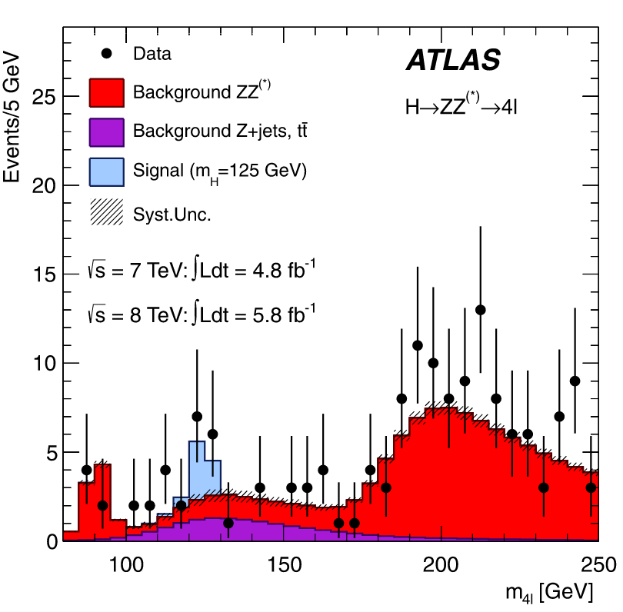
\includegraphics[width=0.6\textwidth]{pic/events.png}
    \caption{Signal at \qty{125}{GeV}.}
    \label{fig:events}
\end{figure}

另一个重要的衰变道是双光子衰变道。相对于其他夸克或胶子等强子对末态,双光子的分支比要小得多,但更容易识别。它的数据是则是由双光子触发判选系统选择的,并且需要在电磁量能器中形成两束光子簇的能量。在能量为 \qty{7}{TeV} 时,每个光子簇的横向能量要大于 \qty{20}{GeV};\qty{8}{TeV} 时,则要分别大于 \qty{35}{GeV} 和 \qty{25}{GeV}。并且由于存在能量损失和能量渗漏,要用蒙特卡罗模拟来修正候选光子的能量。双光子的不变质量则由电磁量能器中测的光子能量、光子在量能器中的方位角 $\phi$ 和初始顶点与碰撞点计算出的赝快度η得出。最终 在 \qty{100}{GeV} 到 \qty{160}{GeV} 的不变质量范围内,在能量为 \qty{7}{TeV} 和 \qty{8}{TeV} 时,分别选出了 $23788$ 和 $35251$ 对候选的双光子。为了提高对希格斯粒子寻找的灵敏度,还将这些事例分成了 $10$ 个种类。这是划分出的种类和对应的事例数量。这里的 $p_{Tt}$ 是双光子横向动量垂直于轴的分量。

\begin{figure}[htbp]
    \centering
    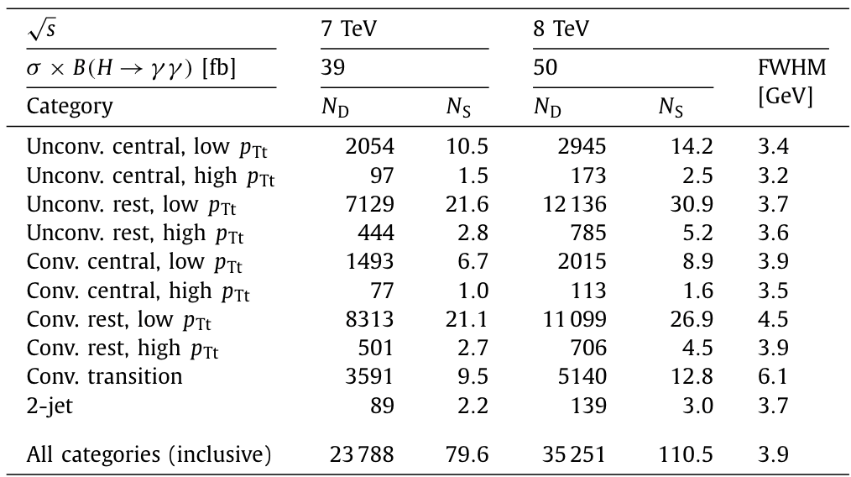
\includegraphics[width=0.6\textwidth]{pic/10.png}
    \caption{$10$ 种事例}
    \label{fig:10}
\end{figure}

双光子衰变道中,主要的本底是标准模型下,高能质子和质子对撞产生的双光子末态,同时还有产生的喷注被误认为光子,以及 Drell-Yan 过程的影响,这是一个产生于高能强子散射的过程。在双光子衰变道的本底预测中,按之前分的不同种类用了不同的处理手段。比如说对某些种类,则用四阶伯氏多项式去预测,而其他的则用指数函数去处理。

最后的结果如图所示,上面的这张红色的,虚线是相对希格斯粒子质量为 \qty{126.5}{GeV} 预测的本底,实线是本底加上希格斯粒子的信号。下面蓝色的则是加权后的情况,这里是将不同种类的数据进行了不同权重的处理。这两个则是将本底扣除的结果。也是能从双光子的不变质量谱上发现一个峰。

\begin{figure}[htbp]
    \centering
    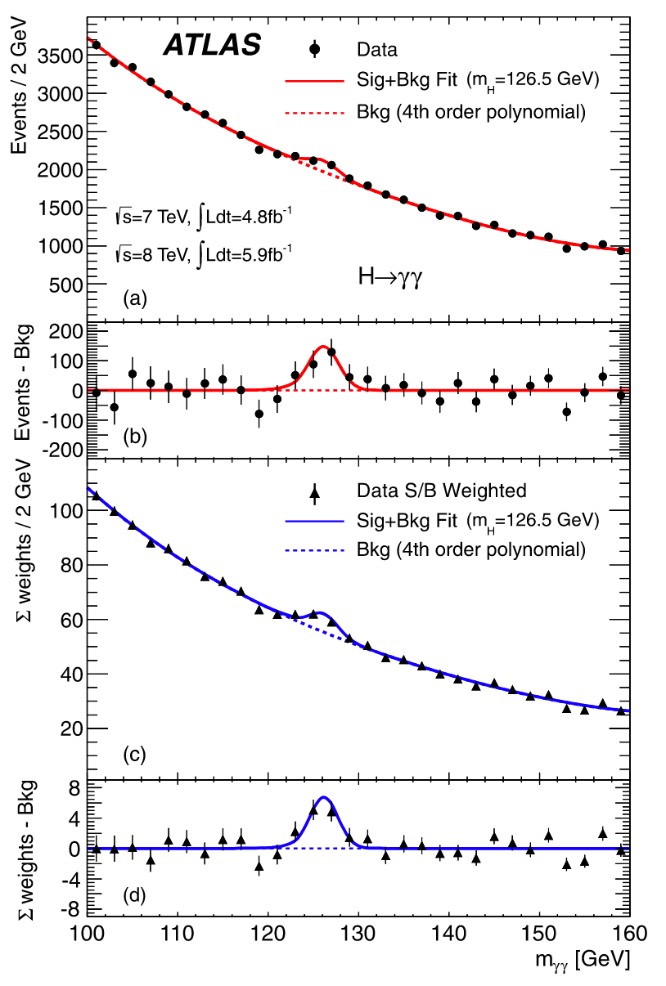
\includegraphics[width=0.6\textwidth]{pic/atlas.png}
    \caption{ATLAS 实验结果}
    \label{fig:ATLAS}
\end{figure}

\section{ss}

通过引入一个信号强度参数 $\mu$,建立模型 $\mu s(m) + b$;

假设检验问题:

\begin{itemize}
    \item 零假设 $H_0: \mu=0$,表示没有信号,只有背景存在;
    \item 备择假设 $\mu > 0$,表示存在一个信号。
\end{itemize}

我们想要检验的是是否存在一个信号强度大于 $0$ 的共振。

模型中的背景分布 $b$ 和信号分布 $s$ 可能还依赖于其他干扰参数,但在这里的表示中被省略了。质量 $m$ 是另一个干扰参数,但在零假设下不存在,因为背景分布 $b$ 不依赖于 $m$。因此,这个检验问题中存在一个只在备择假设下出现的干扰参数。

当搜索范围内可能存在共振时,我们会寻找超过背景的最大事件过剩。具体来说,如果 $q(m)$ 是针对固定质量的检验统计量,并且较大的 $q(m)$ 值表示与零假设的兼容性降低,那么整个范围的检验统计量将是 $q(\hat{m})=\max_m ⁡[q(m)]$,即取所有固定质量下的检验统计量的最大值。

实验中,我们感兴趣的参数是 \emph{全局信号强度因子 (Global signal strength factor)}$\mu$ \footnote{使用基于轮廓似然比的统计量 $\lambda_\mu$ 来测试 $\mu$ 的假设值。该测试统计量从对数据进行的完整似然拟合中提取了信号强度的信息。似然函数包括描述系统误差及其相关性的所有参数。},它作为一个比例因子影响了标准模型中预测的希格斯玻色子信号的总事件数。

排除限制是基于 CLs 方法 \footnote{Confidence Level as a function of the test Statistic} 进行的;当 CLs 小于 $5\%$ 时,我们将 $\mu$ 值视为在 $95\%$ 的置信水平下被排除。当在质量为 $m_H$ 的情况下排除 $\mu=1$ 时,我们认为质量为 $m_H$ 的标准模型希格斯玻色子已经被排除,置信水平为 $95\%$。

对于在给定搜索区域中观测到最显著过剩的全局概率,计算全局概率与局部概率之比——试验因子 (trial factor),用于纠正“look elsewhere effect” \footnote{"Look elsewhere effect"是指在进行多次统计假设检验时可能出现的误导性结果。当进行多个假设检验时,有一定概率会出现某个检验结果达到显著性水平,即使在没有真实效应的情况下也可能发生。}。 统计检验是以假设的希格斯玻色子质量 $m_H$ 的值为步长进行的。

相关系统误差的主要来源如下:

\begin{enumerate}
    \item 累计亮度:累计亮度的不确定性在通道之间被视为完全相关。
        \begin{itemize}
            \item 对于 \qty{7}{TeV} 的数据,它为 $3.9\%$
            \item \qty{8}{TeV} 的数据的不确定性为 $3.6\%$。
        \end{itemize}
    \item 电子和光子触发识别:电子和光子触发和识别效率的不确定性在电子和光子之间被视为完全相关。
    \item 电子和光子能量标度:$H \to ZZ(*) \to 4\ell$ 和 $H\to\gamma\gamma$ 通道中的电子和光子能量标度由五个参数描述,它们详细说明了系统误差的来源。
    \item $\mu$ 子重建:影响 $\mu$ 子的不确定性被分为与内部探测器 (ID) 和磁谱仪 (MS) 相关的部分,以便更好地描述使用不同的 $\mu$ 子鉴别标准和正负电子动量范围的通道之间的相关效应。
    \item 喷注能量刻度和缺失横向能量:喷注能量刻度和喷注能量分辨受到与喷注的 $p_T$、和味有关的不确定性的影响。结果对于关于这些不确定性来源之间相关性的各种假设的敏感性被发现是可忽略的。除了 JES 不确定性外,还包括了一个与未重建的物理对象不相关的低能喷注活动有关的 $E_T^miss$ 不确定性分量。
    \item 理论不确定性:相关的理论不确定性主要影响信号预测。
\end{enumerate}

使用 \qty{8}{TeV} 数据对于 $H\to ZZ(*)\to 4\ell$、$H\to\gamma\gamma$、$H\to WW(*)\to e\nu\mu\nu$ 通道的分析,以及对 \qty{7}{TeV} 数据在前两个通道中的改进,相较于先前的综合搜索,在低质量区域带来了显著的灵敏度提升。

\begin{figure}[htbp]
    \centering
    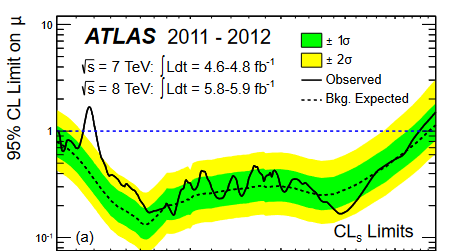
\includegraphics[width=0.6\textwidth]{pic/95CL.png}
    \caption{以 $m_H$ 为函数,展示了以信号强度参数 $\mu$ 表示的标准模型希格斯玻色子产生的置信度排除。}
    \label{fig:mH}
\end{figure}

\begin{itemize}
    \item 在 $95\%$ 置信度排除了从 \qty{110}{GeV} 到 \qty{582}{GeV} 的 $m_H$ 范围。
    \item 在 $99\%$ 置信度下,排除了三个质量区域,分别为 \qtyrange{113}{114}{GeV},\qtyrange{117}{121}{GeV} 和 \qty{132}{527}{GeV} 
\end{itemize}

在 $H\to ZZ(*)\to 4\ell$ 和 $H\to\gamma\gamma$ 通道中观察到了在 $m_H=\qty{126}{GeV}$ 附近的事件过剩,这两个通道都提供了具有高不变质量分辨率的完全重建候选事件。

\begin{figure}[htbp]
    \centering
    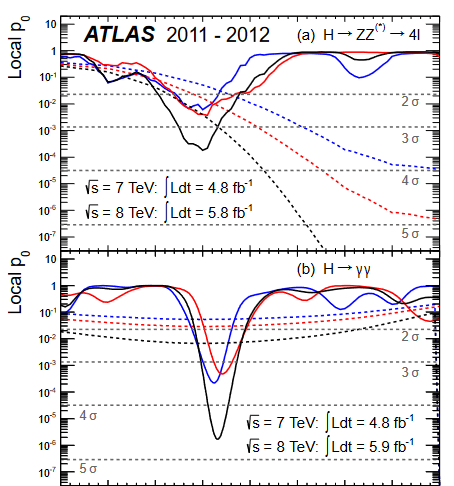
\includegraphics[width=0.6\textwidth]{pic/p0.png}
    \caption{}
    \label{fig:p0}
\end{figure}

在 \qty{7}{TeV} 和 \qty{8}{TeV} 数据的组合中,最大的局部显著性发现在 SM 希格斯玻色子质量假设 $m_H=\qty{126.5}{GeV}$ 处,达到 $6.0\sigma$

这些结果提供了新粒子发现的确凿证据,其质量为 $\qty{126.0}{GeV} \pm 0.4(\text{统计}) \pm 0.4(\text{系统})$。对于以电荷和为零的矢量玻色子对的衰变,确认了新粒子为中性玻色子。

\end{document}
